\documentclass[
    titlepage,
    twoside,
    openright,
    12pt
]{book}

\usepackage{lib/polithesis}

%*****************************************************************
%                         CUSTOM PACKAGES                         
%*****************************************************************

% Should you need to add custom packages, this is the right place.

%*****************************************************************
%                      THESIS CUSTOMIZATIONS                      
%*****************************************************************
%
%   In this section, you can insert the data to be displayed in
%   the title page. If you do not want to show something, just
%   comment it using '%' at the beginning of the line.
%
%*****************************************************************

% Specify thesis language in lowercase (default "english")
\thesislanguage{english}
% Choose the font for the thesis
% The available choices are: "Computer Modern", "Baskerville",
% "Nimbus", "Palatino", "Utopia".
% If an invalid font is set, the fallback font used is the default
% LaTeX font "Computer Modern".
\thesisfont{Palatino}
% Change title color
\titlecolor{MidnightBlue}
% Change color of chapters' number
\chapnumbercolor{ThesisGray}
% The available colors are the 68 dvips colors plus the defaults.
% (https://en.wikibooks.org/wiki/LaTeX/Colors#Predefined_colors)
% You can define you own color as done for ThesisGray in the
% library file, even if it is not recommended.

\makeglossaries
% The form of the entries in this file is \newacronym{label}{acronym}{phrase}
%                                      or \newacronym[options]{label}{acronym}{phrase}
% see "User Manual for glossaries.sty" for the  details about the options, one example is shown below
% note the specification of the long form plural in the line below
\newacronym[longplural={Debugging Information Entities}]{DIE}{DIE}{Debugging Information Entity}
%
% The following example also uses options
\newacronym[plural={OSes}, firstplural={operating systems (OSes)}]{OS}{OS}{operating system}

% note the use of a non-breaking dash in long text for the following acronym
\newacronym{IQL}{IQL}{Independent Q‑Learning}

\newacronym{LAN}{LAN}{Local Area Network}
% note the use of a non-breaking dash in the following acronym
\newacronym{WiFi}{Wi-Fi}{Wireless Fidelity}

\newacronym{WLAN}{WLAN}{Wireless Local Area Network}
\newacronym{UN}{UN}{United Nations}
\newacronym{SDG}{SDG}{Sustainable Development Goal}

% Comment this line if you only want to appear
% the acronyms present in the document
\glsaddall

% Use acronyms in the text with the following commands
% \gls{ }
% To print the term, lowercase.
%
% \Gls{ }
% The same as \gls but the first letter will be printed in uppercase.
%
% \glspl{ }
% The same as \gls but the term is put in its plural form.
%
% \Glspl{ }
% The same as \Gls but the term is put in its plural form.
%
% \acrlong{ }
% Displays the phrase which the acronyms stands for. Put the label of the acronym inside the braces.
%
% \acrshort{ }
% Prints the acronym whose label is passed as parameter.
%
% \acrfull{ }
% Prints both, the acronym and its definition.                 %load the acronyms file

%*****************************************************************
%                         TITLE PAGE DATA                         
%*****************************************************************
%
%   In this section, you can insert the data to be displayed in
%   the title page. If you do not want to show something, just
%   comment it using '%' at the beginning of the line.
%
%*****************************************************************

\university{Politecnico di Milano}
\faculty{Facoltà di Ingegneria}
\school{Scuola di Ingegneria Industriale e dell'Informazione}
\department{Dipartimento di Elettronica, Informazione e
 Bioingegneria}
\course{Computer Science and Engineering}
\title{A Fancy Title\\for a Fancy Thesis}
\supervisor{Prof.ssa Franca Garzotto}
% You can specify more than one co-supervisor, separating them
% with commas.
\cosupervisors{Ing. Alberto Patti, Ing. Francesco Vona}
% Each author should be added as a tuple of her name and her
% matriculation number joined with a comma.
% You can specify more than one author, separating each one with
% a comma. They will be printed in different lines.
\authors{Fabiana Ferrara, 944373, Stefano Formicola, 953554}
\matriculationPrefix{matr.}
\academicYear{2020/2021}

%*****************************************************************
%                         THESIS CONTENT                         
%*****************************************************************
\begin{document}

% Title Page
\maketitle

% Optional, comment or delete instruction to remove
\dedication{Insert here your dedication.\\Optional.}

% Chapters
\frontmatter
\pagenumbering{Roman}
\chapter{Abstract}

Nowadays, existing approaches for creating Extended Reality (XR) experiences mostly entail the use of Integrated Development Environments (IDEs) or software libraries (APIs), while the adoption of a high-level approach -- allowing to abstract from the implementation -- is however confined to technology-dependent methods or close descendants of standard meta-models.
What is needed, therefore, is a universal model that allows XR applications to be designed at the conceptual level, without relying on solutions that are domain-specific or that exclude non-programmers from designing. This thesis presents the XRM Model, a theoretical approach oriented towards the conceptualisation of XR experiences, developed from a comparative study of existing models in the literature. The XRM Model is adopted for the implementation of a High-Level Editor to support XR application designers, which was validated in a usability test with users based on the ISO 9241-11 standard. In conclusion, an experience designed for an archaeological complex was considered as a case study in order to show the benefits resulting from the adoption of the XRM and the ART Editor.


\paragraph{Keywords}  Human-Computer Interaction; Interaction Design; Extended Reality; Conceptual Modelling; Authoring tools; Tourism; Cultural Heritage
\chapter{Sommario}
Al giorno d'oggi gli approcci esistenti per la creazione di esperienze in Exted Reality (XR) consistono nella maggior parte dei casi nell'utilizzo di ambienti di sviluppo integrato (IDEs) o librerie software (APIs), mentre l'adozione di un approccio ad alto livello -- che consenta di astrarre dall'implementazione -- è tuttavia limitato a metodi dipendenti dalla tecnologia o stretti discendenti di meta-modelli standard.
È necessario, quindi, un modello universale che permetta di progettare a livello concettuale applicazioni XR, senza ricorrere a soluzioni che siano strettamente dedicate al dominio o che escludano dalla progettazione i non esperti di programmazione. In questa tesi viene presentato il Modello XRM, un approccio teorico orientato alla concettualizzazione di esperienze XR, sviluppato a partire da uno studio comparativo dei modelli esistenti in letteratura. Il Modello XRM è stato adottato per l'implementazione di un Editor ad alto livello a supporto dei designer di applicazioni XR, il quale è stato validato in un test di usabilità con utenti basato sullo standard ISO 9241-11. In conclusione si è considerato come caso di studio un'esperienza progettata per un complesso archeologico allo scopo di mostrare i benefici risultanti dall'adozione dell'XRM e dell'ART Editor.


\paragraph{Parole chiave} Human-Computer Interaction; Interaction Design; Extended Reality; Conceptual Modelling; Authoring tools; Tourism; Cultural Heritage
\chapter{Acknowledgements}

We would like to thank the company Fifthingenium S.r.l.s for the opportunity they gave us to work on this thesis project. 

Special thanks to Luigi Oliveto who supervised us during the entire project in the company. 

We would like to extend special thanks to Prof. Garzotto, and to co-supervisors Ing. Patti and Ing. Vona who supported us in the various aspects of the master thesis with great humanity, commitment and dedication.
\thesistoc

%*****************************************************************
%                            CHAPTERS                            
%*****************************************************************

\mainmatter
\chapter{Introduction}

\section{Context}
The Covid-19 pandemic situation has negatively impacted the tourism and events business sectors and thus the economy of many cities in Italy, strongly dependent on this sector.
ART (Augmented Reality for Tourism) is a project aiming at offering an innovative Extended Reality (XR) toolset to build services targeting the tourism sector, starting from the Italian market.
Thanks to solutions developed in ART, XR services and experiences will become more accessible and economically feasible, offering tourism actors a way to be more resilient to an emergency situation and safer experiences to their visitors.
Thanks to this framework, despite the current limitations regarding gatherings of people, the attractiveness of a city and its touristic points of interest will be partly supported by those actors that will invest in XR technologies, digitizing their assets and offering multiple experiences for visitors during their digital journeys, both while connecting remotely and while visiting physically.
The ART project will enhance visitors’ experience while simplifying the authoring work for the service provider. The project aims at developing a XRaaS platform, or XR as a Service, offering the opportunity to easily create multi-device XR applications starting from existing 3D models. It is mainly meant for small-medium businesses, without expertise in developing XR applications, who want to offer immersive experiences to their final customers. To achieve this, the main feature of ART will be the capability of linking the 3D content to the real world using XR helmets and a specific authoring application.

The ART project\footnote{\url{https://outoftheframe.art}} is funded by EIT Digital\footnote{\url{https://www.eitdigital.eu}} with the strategic partnership of companies as Telecom Italia (TIM) and FifthIngenium S.r.l.s.\footnote{\url{https://fifthingenium.com}} and the academic collaboration of Technische Universität Berlin (TUB) and Politecnico di Milano. This thesis is the result of the authors' work based on a company internship at Fifthingenium. 
The internship lasted 4 months during which, in a first phase, we focused on the study of XR technology and its components with the aim of designing and iteratively refining a conceptual model with all its features, and in a second phase, we contributed to the creation of an online editor designed for XR experiences.
The company also provided us with some projects, examples of real case studies that could help us define our model. 

The NURE experience is the case study used in this thesis to validate our proposal. 
NURE\footnote{\url{https://www.nurearcheologia.it}} is an organisation that was created to supply integrated services for archaeology; it is a production and work cooperative established in 2010 and based in Isili (SU), Sardinia. For almost ten years it has been involved in the management of archaeological excavations and museums, archaeological surveys, scientific assistance in restoration and conservation consolidation of monuments, preventive archaeology, cultural heritage education, museum design and layout, and the valorisation, promotion and management of archaeological sites and landscapes. 
NURE is responsible for the archaeological area of Santa Lucia di Assolo (OR), a very interesting multi-layered site that preserves important traces from the Bronze Age to the Middle Ages, with the ruins of an imposing polylobate nuraghe with its village (XIV-IX century BC), a terma, a road and several dwellings from the Imperial Roman period (III-IV century AD). There is also a Paleochristian sepulchral area with numerous tombs and a patrician funerary mausoleum located in the immediate proximity of the church, which was originally built in the Byzantine period (7th century).
In collaboration with NURE, we contributed to a Mixed Reality Musealization project of the archaeological area located in Santa Lucia di Assolo (OR), whose aim was to "revive" some very ancient archaeological sites thanks to the use of recent XR technologies.


\section{Research Questions}
An increasing trend on XR applications has been found in the last years, however literature lacks research into development of high-level design tools abstracting from the implementation, resulting mostly in tailor-made techniques. A non-technology dependant model is needed in order to allow the development of cross-reality experiences and let designers focus on relevant aspects as structural, behavioural and interaction, reducing time and resources in communication efforts within the team. At the same time, a lack of technical expertise -- usually required by traditional development environments -- prevents authors from building the experience. Therefore this work aims at answering the following research questions:
\begin{itemize}
    \item[RQ.1]\emph{What design characteristics of Extended Reality (XR) are useful, and how can they be modelled by structural, behavioral and interaction properties in a human-centered designed conceptual framework?}

    \item[RQ.2]\emph{Can a High-Level Authoring Tool facilitate the creation of XR experiences for non-expert people? What are the benefits in terms of effectiveness, efficiency and satisfaction as measured by qualitative and quantitative data?}
\end{itemize}

We answer these questions proposing an innovative and flexible conceptual model to describe XR experiences whose its submodels have the goal to define the appearance and properties of the entities -- including the user -- that structure the application, their behaviour and their resulting perceivable changes of initial properties in order to compose the activities that the user can address within the experience. In addition to this, we adapted the proposed conceptual model in the frame of the ART project guiding the development of an editor to support the authoring of XR experiences.

\section{Research Methodology}
A preliminary study of the literature allowed to understand the context and its state of the art. Several searches on the academic search engine Google Scholar have been carried out to guide the review proposed in the next chapter and structured as follows:
\begin{enumerate}
    \item A first query was related to XR and its role in tourism in the time range 2015-2020:
        \begin{itemize}
            \item \texttt{((virtual OR mixed OR augmented OR extended) AND reality) AND (cultural heritage OR tourism)}
        \end{itemize}
        After a filtering based on titles and, later on, abstracts, we selected 48 papers to review resulting in 44 useful works that guided our study.
    \item The second set of queries aimed at searching for conceptual models or modelling techniques in XR or its specifications:
        \begin{itemize}
            \item \texttt{(((design  AND methods )  OR  (conceptual  AND  (model  OR\\ models))) AND (XR  OR  MR))} in the year range 2015-2021.\\
            22 papers have been selected for further readings, that resulted in 7 relevant articles to examinate.
            \item \texttt{"conceptual modeling" OR "conceptual model" intitle:AR\\ OR intitle:"augmented reality" OR intitle:"mixed reality"} in the year range 2015-2021.\\
            Resulting in 4 works selected.
            \item \texttt{"multimodal interaction techniques" AND " ("VR" OR "AR") "} in the year range 2005-2021.\\
            10 articles found for closer examination, 2 of them have been taken in consideration for a literature review.
            \item \texttt{intitle:"modeling 3D Content" OR  intitle:"semantic\\ modeling" AND (VR OR AR OR MR)}\\
            10 articles have been selected and read, resulting in 4 relevant works accepted.
            \item Other articles have been considered based on their similarity with the topic or through citations found in the above mentioned works.
        \end{itemize}
    \item The last set of queries investigated on advances and works of the last 4 years (2018-2021) in the field of authoring tools and relevant IDEs and APIs, to offer an overview of the current platforms used in the AR/VR development field:
        \begin{itemize}
            \item \texttt{intitle:"augmented reality development" OR intitle:"AR\\ development" OR intitle:"AR framework" OR intitle:"AR\\ frameworks" OR intitle:"Augmented Reality framework" OR intitle:"AR tools" OR intitle:"Augmented Reality framework"}\\
            Starting from 113 results, only 2 papers have been chosen given the relevance with our intended research, filtering them by title, keywords and abstract.
            \item \texttt{intitle:"virtual reality development" OR intitle:"VR\\ development" OR intitle:"VR framework" OR intitle:"VR\\ frameworks" OR intitle:"Virtual Reality framework" OR intitle:"VR tools" OR intitle:"Virtual Reality framework"}\\
            Starting from 109 results, only 4 papers have been chosen given the relevance with our intended research, filtering them by title, keywords and abstract.
            \item \texttt{intitle:"authoring" OR intitle:"SDK OR SDKs" AR\\ augmented VR virtual reality}\\
            Resulting in 98 results, of which 13 papers have been selected for further reading given their relevance with the research.
            \item Other articles have been considered based on their similarity with the topic or through citations found in the above mentioned works.
        \end{itemize}
\end{enumerate}

\section{Thesis outline}
The thesis is structured as follows: \autoref{ch:background} provides an extensive review of the state of the art on XR technologies and their applications in tourism, an overview and comparative study on the existing conceptual models in XR (\autoref{sec:background-conceptual}) and, in conclusion, a thorough analysis on authoring tools in XR (\autoref{sec:background-authoring}).

The next chapter propose the XRM Conceptual Model and its sub-models: the structural (\autoref{sec:conceptual-structural}), behavioural (\autoref{sec:conceptual-behavioral}) and interaction (\autoref{sec:conceptual-interaction}) models and their application on a concrete use case (\autoref{sec:conceptual-nure-example}). 

Subsequently, \autoref{ch:art} describes the ART Framework and focuses on the implementation of the ART Editor (\autoref{sec:art-editor}) based on a high-level and low-level design process and validated on the same use case found in \autoref{sec:conceptual-nure-example} (\autoref{subsec:art-editor-nure-example}). 

An experimentation phase followed the editor design, resulting in the definition of a usability evaluation study (\autoref{ch:evaluation}) and -- consequently -- the analysis of results (\autoref{sec:evaluation-results}).

Finally, in \autoref{ch:conclusions} the concepts expressed within the thesis are summarized, and the main open challenges in the field are indicated.
\chapter{Background}
\label{ch:background}

\section{Extended Reality}
\label{sec:background-intro}

\gls{XR} is an umbrella term encompassing all the possible combinations of real and virtual environments included in the spectrum of the \emph{Reality-Virtuality Continuum} (see \autoref{fig:virtuality-continuum}), introduced by Paul Milgram and Fumio Kishino in 1994 \cite{milgram_taxonomy_1994}.

\begin{figure}[h]
	\centering
	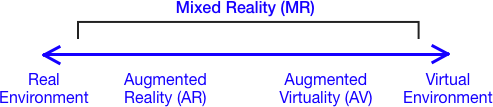
\includegraphics[width=7.5cm]{Background/virtuality-continuum.png}
	\caption{Milgram and Kishino's “Reality-Virtuality Continuum”}
	\label{fig:virtuality-continuum}
\end{figure}
In their work, the authors considered the real environment and \gls{VE}, also known as \gls{VR}, as two sides belonging to the same continuum, instead of two words in antitheses. Between them there exist other concepts with a variable quantity of real and VE such as \gls{AR} and AV. AR allows users to see the real world with virtual objects superimposed upon it, while with AV is the real world that augments the virtual environment. \gls{MR}, instead, has the peculiarity of mixing these two concepts, creating experiences in which physical and virtual objects co-exist and interact in real time with the user.

Some more emphasis on AR is put by Ronald Azuma \cite{azuma1997survey}, where the author defined three academic criteria for AR: it \textit{“combines the real and virtual”}, it is \textit{“interactive in real time”} and it is \textit{“registered in three dimensions”}. Later, Azuma et al.~\cite{azuma2001recent}, added that AR's objective is to \textit{“enhance the user’s perception of and interaction with the real world”}.

From this introduction it is clear that the “X” of XR represents a variable for any of these existing combinations. We have Augmented Reality (X=A, AR), Mixed Reality (X=M, MR) and Virtual Reality (X=V, VR). XR not only covers these environments but, as Honkanen \cite{honkanen_enhancing_2018} states, it is also the common term representing their immersive technologies and \textit{“human-device interaction aspects”}. Suh and Prophet \cite{suh_state_2018}, in their literature review on immersive technologies, describe XR as a means through which users' reality is extended as they feel placed within a simulation where real and simulated environments are indistinguishable \cite{kwok_covid-19_2020}.

A technical background of AR and VR is given by Egger et al.~\cite{egger_augmented_2020}. Generally, the main steps to produce AR experiences are twofold \cite{jenny_enhancing_2017}.
Content or landmarks indicating where AR is to be applied are detected in a first step. Subsequently, virtual objects are added above the camera feed based on the previously detected references \cite{parker_jr_augmented_2014}. Through the visors, devices equipped with a camera that captures the frames, it enables to see the AR information automatically i.e. without manual activation. In order to enable the device to recognize the real environment, the position of the user and what they are looking at, tracking must take place.Through the use of markers (\emph{marker-based} tracking), two-dimensional printed objects, objects in the real world are taken as landmarks. These identifiable elements can be scanned, so that the application software can interpret them and place the augmented objects or obtain information without using the geolocation. \emph{Marker-less} tracking) allows the use of sensors, such as accelerometer, cameras, GPS, to create anchor points based on recognisable features of the surrounding environment. \cite{egger_augmented_2020}.
Orthogonally to the tracking system used, another dimension to consider is the way we can experience AR:
\begin{enumerate}
	\item \glspl{HMD}, or “see-through AR glasses”, are a wearable device that work as normal glasses and contemporaneously have a small projector on the lenses to augment the real world with additional contents. The real environment is captured by the users by freely moving around it.
	\item Handheld devices equipped with all the components needed to record the real world and track its objects, e.g. camera, accelerometer and GPS. Most smartphones are equipped with these built-in instruments making AR widely used.
	\item Other forms of displays that do not belong to the Mobile AR (MAR) category (i.e. the two categories described above). An example of these displays are the AR mirrors often placed in open spaces that \textit{“do not require users to depend on any kind of device or application to experience AR”}.
\end{enumerate} 
VR, on the other hand, renders a totally VE that can be navigatd and interacted by the users, which one or more of their five senses are simulated in real-time \cite{guttentag_virtual_2020}. The author's study also defines two characteristics of VR: the ability to provide a physical immersion and a physical presence, making participants behave as in a real-life situation.
The VE, as explained by Egger et al., can represent either a computer-generated world or a 360$^{\circ}$ real-captured video or image.

Beck et al.~\cite{beck_virtual_2019} classify VR systems (VRs) distinguishing between non-, semi- and fully immersive VRs. The first term classifies desktop solutions allowing to navigate 360$^{\circ}$ videos and images in a classical PC interaction through mouse and keyboard. They are the simplest and most used form of VR, in platforms like YouTube and Facebook 360$^{\circ}$ Video. Semi-immersive systems have been used in the past years by projecting screens onto the walls and floor of a room and complementing the setting with spatial sounds, allowing a multi-user experience.
Fully immersive VRs, instead, require users to wear a \gls{HMD} that supports head tracking and other interactions through controllers or wearable devices, with the resulting feeling of a complete embodiment in the Virtual Environment.

Jung and Jeong \cite{jung_classification_2020} provide a further classification of VR devices according to the physical connectivity, tracking system and user behavior. Based on the physical connectivity there exist 4 categories that classify a VR device:
\begin{itemize}
    \item PC-tethered VR, Console-tethered VR: a VR headset connected to a desktop computer and a video game console that render the VE;
    \item Standalone VR: it is simply made by an untethered headset;
    \item Smartphone VR: a system made using a smartphone to render the graphics and a headset with lenses to recreate the VR effect.
\end{itemize}


In terms of tracking systems two technologies are used to track user's motion, the head tracking and position tracking: the latter uses the internal sensors of the headset (e.g. gyroscope, accelerometer and magnetometer), the former can be again divided into inside-out position tracking, which uses the camera on the headset to determine the movement, and outside-in position tracking that relies on external devices.
For what concerns user behavior categorization, VRs are divided into stationary VR, desktop-scale VR, room-scale VR and mobility VR. A VR device that does not have a position tracking feature can only be used in a stationary way, belonging to the stationary VR category; the desktop-scale VR and room-scale VR are opposites and refer to, respectively, systems with a restricted position tracking coverage and systems with a wider one. With a mobility VR device the user does not have space constraints and can, therefore, use it without spatial restrictions given its untethered nature and stand-alone position tracking component.
\section{XR in Tourism}
\label{sec:background-tourism-xr}

%Over the years, XR has been used to offer new ways to interact with the surroundings in many different fields such as medicine, industry, rehabilitation, etc. %
The market for XR applications today includes growth sectors including health and military technology that have been growing for a while, compared to other types of applications that are only recently gaining ground \cite{honkanen_enhancing_2018}. The tourism industry is one of the latest commercial applications that offers incumbents new opportunities to expand their business and the XR companies they partner with to become tourism experts \cite{kwok_covid-19_2020}.
Until recently, cultural tourism represented little more than a niche market \cite{han_virtual_2019}, with the traveler's experience being limited to site-related activities only. It was predictable that it would become an important economic and social driver in Europe and worldwide as visitors' engagement and the learning experience increased. Han et al.~\cite{han_virtual_2019} argue how technology can open up new opportunities to reformulate the user experience. On the other hand, Bekele et al.~\cite{bekele_survey_2018} discuss the significant added value that cultural heritage sites and artifacts gain from the introduction of technologies such as AR and VR.

For what concerns the application of XR in tourism and Cultural Heritage (CH), there are multiple examples of them as evidenced in Bekele et al.~\cite{bekele_survey_2018} and Loureiro et al.~\cite{loureiro_20_2020}. Several areas, all of crucial importance, can be addressed by an innovation as the one mentioned above. Such technologies are perceived as a powerful educational but also entertainment tool, of high utility if one considers the possibility of language translation, navigation, booking and so on. The resulting benefits impact not only the final user but also local attractions and their business growth \cite{nayyar_virtual_2018}. 

\subsection{Acceptance of immersive technologies in tourism}
Many studies highlight the advantages of exploiting these technologies, considering their limitations and how much people are willing to switch from a more common type of experience to an XR one.
The studies conducted by Kim et al.~\cite{kim_empirical_2020} reveal empirical proofs in support of the last sentence. The model they propose shows that interactivity, experience-ability and amplified engagement are the three main strengths of AR and VR contents.  

Despite all the possible benefits, it is still necessary to consider also how people might react to XR. Some people might be interested or curious while others might prefer a traditional kind of trip. The feedback is usually different based on how accustomed users are to new technology: people more familiar with it are more willing to try and they are more concerned about the quality of the system. Those who have never had a chance to try it or have little to no knowledge are more concerned about the quality of the content \cite{bulchand-gidumal_tourists_2020}, \cite{pourfakhimi_acceptance_2020}.

Referring to the behavior of the user approaching a technology in a friendly manner is the acceptance whereas when referring to the adoption of a technology the focus is on the reasons for adopting it. The extensive research in progress by Pourfakhimi et al.~\cite{pourfakhimi_acceptance_2020} aims at exploring the thoughts, emotions, interactions and impacts of a user or a possible user who is motivated or willing to buy, use and interact with a technology, without omitting examples of tourism-related technologies such as VR.

During the so-called “decision phase” of a customer, it is determined whether or not the barriers of adopting a new technology will be broken through. According to Laurell et al.~\cite{laurell_exploring_2019}, in order to overcome these barriers and thus encourage the diffusion of technology itself, one has to rely both on its autonomous value and, above all, on the perceived value of the technology. This will have to be greater than the overall value related to the utility it brings to the individual (i.e. if it is easy or fun to use), the number of users already using it and the “availability of complementary goods of the old technology”. 

However, this is not the only limitation to be considered, since as with any technology in its infancy, XR is subject to some restrictions such as the duration of use, not to mention that it offers an experience which, even if it comes close to the real world, has a feeling of artificiality. Faced, though, with another type of constraints such as those imposed by the COVID-19 regulations, what might previously have been perceived almost as a threat becomes an asset \cite{guttentag_virtual_2020}. Virtual tours have experienced a surge since they were the only way to enjoy cultural experiences. An opportunity, if you can call it that, that has the responsibility to be up to the level of the original places being reconstructed in VR, as they might positively or negatively influence the user to visit a place in the near future. 

%Travel phases (qui o prima di TAM??)
\subsection{XR in Travel Industry}
What was seen in Bekele et al.~\cite{bekele_survey_2018} was then also found in other research works comparing the above results with those obtained in other applications and implementations, not only in a CH context but considering every step of the tourist journey. For example, Bulchand-Gidumal et al.~\cite{bulchand-gidumal_tourists_2020} divided the user journey in three main phases:
\begin{enumerate}
	\item the pre-travel where the user starts planning the trip, developing the expectation;
	\item the travel where the user experiences the planned trip;
	\item the post-travel where the user shares and re-experiences the journey.
\end{enumerate}

The research proves how AR and VR can be used in the different stages of travel, as a complement to and augmentation for a travel process or as a substitute to the tourism experience, allowing tourists to enjoy an experience without travelling. In the results of their study VR seems to be more appropriate for pre-travel and post-travel, while AR seems to be a good fit to use during the trip. VR in fact, can be used in the decision-making process, providing tourists a first glance of the destination and the potential activities. Moreover, VR can help planning in advance all the activities of a trip (e.g. getting information on the accessibility of a destination) or booking the accommodations and the activities themselves. This is thanks to key elements of VR (immersion, interactivity, presence) and the possibility to recreate, through 3D contents or 360$^{\circ}$ videos, a totally realistic environment. 
In the post-travel phase VR allows to share and enjoy 360$^{\circ}$ images and videos recorded during a trip, with a word-of-mouth effect on VR-enabled platforms.
In contrast to VR, where immersion in a virtual world is a desired feature, the goal of AR is to enhance the way in which the users perceive the real world, by adding layers of virtual objects. Therefore, they agree that Augmented Reality can provide tourists enhanced information on the sites, for example showing users how a certain site looked like at a different point in history, or a way to buy product and services while visiting a destination.

In Egger et al.~\cite{egger_augmented_2020} a comprehensive description of how AR and VR can be implemented in the tourism marketing is given. Before booking a travel AR can augment brochures, flyers, websites and flight tickets to boost the storytelling for a brand, while VR is essential to preview parts of a journey in a “try before you buy” experience. During the trip, POIs can be suggested by an AR application and CH sites are enhanced with additional information or narratives, adding a gamification and storytelling layer. On the other hand, virtual walks substitute inaccessible locations or not existent sites.

Some concrete examples of XR experiences in the industry are given by Jenny \cite{jenny_enhancing_2017}. The Finnish airline Finnair created an immersive and interactive VR visit of their new air fleet to showcase the wide seats, large windows and ambient lights; the shipping operator Finnlines, instead, used 3D photo tours to advertise their renovated vessels for ferry trips. The hotel chain Marriott in cooperation with Samsung created the \textit{VRoom Service} for their customers, giving the opportunity to visit multiple countries from their rooms and order food and beverages to the room service. The same company uses VR to provide virtual tours of their accommodations and promote the booking process \cite{adachi_using_2020}; the Hub Hotel in England used AR to render maps of the city on the walls of the rooms, while through the Holiday Inn experience it is possible to see virtual images of famous people at various points \cite{ercan_examination_2020}.

Other researchers like Adachi et al.~\cite{adachi_using_2020} studied and confirmed the effectiveness of VR headset among different media types, stating that an \gls{HMD} acts on the self-presence feeling of a user, increasing their desire for a destination, as also confirmed by Kang \cite{kang_impact_2020} and Leung et al. for hotel VR commercials \cite{leung_fad_2020}.

\subsection{XR for Cultural Heritage}
% Altri titoli:
% Review of previous XR applications in cultural tourism
% A review of XR (applications) for Cultural Heritage
% examples of MR apps...
Bekele et al.~\cite{bekele_survey_2018} examined augmented, virtual, and mixed reality from a cultural heritage perspective. They focused on technical aspects such as tracking and registration, VE modeling, presentation, tracking, input devices, interaction interfaces and systems. Notwithstanding them, their overview likewise breaks down the different application zones for XR in CH, namely: education, exhibition enhancement, exploration, reconstruction, and virtual museums.

The creators propose that a definitive decision of enabling technology should rely upon the experience that an application is expected to give. Even though augmented, virtual and mixed reality can be used interchangeably to achieve same purposes, their results show that AR is preferable for exhibition enhancement. Similarly, VR seems better for virtual museums, and mixed reality most viable for both indoor and outdoor reconstruction applications.

\subsubsection{Indoor and outdoor XR applications}

The spatial setting for exhibiting virtual and augmented representation is binding. The design for environments such as museums, galleries and heritage sites hinges on the power to build and tell stories that settle in mind and become knowledge. The visitor must feel involved, not only with their body, but also by moving and interacting with the scene, in order to overturn the figure of the passive observer. Pedersen et al.~\cite{pedersen_more_2017} explain that holographic reality with a 3D point of view is able to impress a feeling of depth and solidity that is quite close to reality. Sometimes the actual content of the museum itself becomes the author of the narrative, immersing the visitor in the museum scene and tour. Once the points of interest have been set, a visit route is designed which takes visitors back to the past. This becomes a great opportunity for locations such as museums, which take on a new role by merging the value of heritage with technological elements that bring innovation, learning through experience and entertainment. The model developed by Trunfio and Campana \cite{jung_augmented_2020} brings the interaction between the different actors involved such as the visitors, the services offered by the museum and the employment of new technologies such as mixed reality. Investing in museums also means contributing to the preservation of cultural and artistic heritage, improving the visibility of the museum and defining new business scenarios.
To experience mixed reality indoors, sometimes you don't even have to travel far. That is the case with the Ascape application that allows to be immersed in the experience of a real tourist while staying at home \cite{cranmer_understanding_2016}. Thanks to the use of 360$^{\circ}$ videos it is possible to explore places from different perspectives. When it comes, instead, to influencing users to visit through an internal preview of the location, it is preferable to adopt \gls{HMD}, the customer has the feeling of “being there” and has a definite intention to visit that place.

%outdoor
Outdoor applications are more suitable for a reconstruction approach, because it is then possible to overlay reconstructed historical views over the real world in a “real-virtual” representation. Complementary, two forms of blended 3D assets are needed when reconstructing cultural heritage in a MR application: present and past views \cite{bekele_survey_2018}. Moreover, a reconstruction theme is often applied to outdoor sites that have been demolished or worn away. When it is not synonymous with extension, it is known as “diminished reality”: virtual elements are removed to restore a scenario to its original state of appearance \cite{honkanen_enhancing_2018}. 
The majority of applications serve virtual museums, followed by education, reconstruction, and exploration purposes.
%HMD, desktop, and CAVE displays are the common choices for displaying a virtual environment. 
In some cases it is convenient to think of outdoor locations, even very wide ones, as museum exhibits. Outdoor environments are more dispersive, but as mentioned before, one of the goals of mixed reality applications is exploration. Therefore it might be relevant to guide users towards the place they are looking for \cite{jenny_enhancing_2017} or to drive them to discover sites they have not visited yet. Exploration is more related to tangible resources of cultural heritage, while reconstruction also uses intangible resources or both, combined to overlay augmented and virtual elements on top of reality \cite{bekele_survey_2018}. According to the location's requirements, it can be decided whether to use the involved technology aiming at replacing reality or at being complementary to it \cite{racz_virtual_2019}. In the first case, it may be a real constraint due to the inaccessibility of some places that are moved into a virtual world to be available. This is also referred to as historical-cultural events. In the latter case, it can be an entertainment and promotional tool for the site to arouse the interest of visitors.
Some examples of AR experiences applied to urban or touristic-cultural contexts demonstrate the superiority of outdoor realism and involvement over indoor, precisely because outdoors favors the use of \gls{HMD} cameras and therefore of AR/VR content \cite{iacoviello_holocities_2020}. Visiting a city is no longer a one-to-one relationship with the mobile application, but it becomes a co-participation, it changes the point of view of the observer visiting that place and becomes an experience that the user shares with nature and art and sometimes with other users.
If indoor cultural tourism exploiting mixed reality has some limitations such as the field of view of \glspl{HMD} that forces the user to always stand at a certain distance from objects thus avoiding that they appear larger than expected, outdoor tourism is even more insidious. A big and still open challenge, in indeed, is the excessive natural light that could limit the view through the viewers and the instability of the building recognizer that allows the virtual reconstruction \cite{debandi_enhancing_2018}. Furthermore, outdoor tracking is always less accurate than indoor tracking. MAR applications need to consider that objects might move slightly or flutter. Building scenarios with AR content requires a great deal of effort, due to the need to customize 3D objects for the specific outdoor space. This implies two challenges identified by Xu et al.~\cite{xu_exploring_2018}, one related to the costs that become demanding and the other related to the immersion in an external environment. The risk, in fact, is to bump into real objects because of the feeling of being completely absorbed in the AR experience.

%distinction physical-remote (?)
So far visitors or users have been identified without specifying whether or not they were physically present at the site of interest \cite{gaberli_tourism_2019}. The new digital era has made it possible for everyone to be a citizen, or rather a tourist, of the world. Being able to visit and learn about places remotely, through the use of the Internet, initially broadened the horizons for all those who could not physically travel. Subsequently, it became a tool for exploring a destination even before arriving there. With the introduction of XR technologies, a new shape of tourism has spread, which has also become very successful from an entrepreneurial point of view. Remote tourism has become a resource for those who intend to travel and those who unfortunately cannot. The remote experience has reached significant levels of popularity, travel communities are a source of information and the number of travel video log views exceeds one billion \cite{adachi_using_2020}. Despite this, there is no comparison between a computer display showing a 360$^{\circ}$ video and the feeling of real presence offered by an \gls{HMD}. Also from a promotional point of view, the headset has a superior persuasive effect due to the quality of the social presence that provides the virtual and augmented environment with an appearance of humanity.
%Museum categorization/virtual museum 
Online museum experiences are explored in depth by studies conducted by Doukianou et al.~\cite{doukianou_beyond_2020} revealing, that they are not very popular, so they should be defined as almost obsolete tools. Virtual museums are presented as a brochure version for promotional purposes and as a collection of contents for educational purposes. The aim is to encourage visitors to come back and repeat the museum tour. It becomes very difficult to invest in such visits if the user experience is not appropriate. In some cases virtual museums include serious games that try to tell a story and increase the value of the experience. %In spite of this, the percentage of visitors who say that museums in their proximity are not embracing technological and innovative solutions is close to 36\%, which says a lot about the interaction of users with such technologies.

\subsubsection{Examples}

There are a lot of examples of AR applications in tourism and cultural tourism. The first MAR app specific for the tourism industry was \textit{Tuscany+}, published in 2010, a digital tourist guide in different languages offering information about sightseeing, accommodations, restaurants and other point of interest for travelers \cite{kounavis_enhancing_2012}, \cite{nayyar_virtual_2018}. Similar applications emerged in the following years: the \textit{StreetMuseum} app, developed for the Museum of London, allows to see historical pictures and additional information of specific places by pointing the smartphone towards streets and buildings. Other MAR apps also offer adventures for users as for the case of \textit{Urban Sleuth} where a multiplayer VE is mixed with the real one in order to solve mysteries by collecting hints exploring a city, its neighborhoods and historical sights \cite{kounavis_enhancing_2012}. A similarity between this kind of apps and the famous AR game Pokémon Go has been found by Nayyar et al.~\cite{nayyar_virtual_2018} where the authors believe that strategically placed “PokeStops” in relevant sights can strengthen the overall tourist experience, as implemented in \textit{Get to Know Moscow} \cite{honkanen_enhancing_2018} where the user is looking for historical characters.
% Gaming experience
Different examples in the literature show the adoption and effectiveness of a gamified AR experience set in historical attractions. Honkanen's Master Thesis \cite{honkanen_enhancing_2018} suggests and implements a double user experience solution in a cultural heritage application: a gamified version for competitive users, and a standard version for non-competitive ones. The former enhances the attraction through an AR storytelling taking place in the past and with the users trying to solve some questions. Users who win the game have the chance to show their name on the leaderboard. Linaza et al.~\cite{linaza_interactive_2007} prototype and test an AR application based on a board game enhanced by augmented cards and virtual avatars guiding the user throughout historical events; their article also provides a useful and detailed reference to design an interactive experience on a historical event based on well-known game dynamics.

Some authors have approached and analyzed the phenomenon of tourists' experience enhancement through MAR. Mobile AR apps act as a digital tourist guide “on-demand”, displaying content upon request and by travelling around the city \cite{kounavis_enhancing_2012}, adding \textit{"a layer of guidance, content and entertainment to physical locations seen through the smartphone's camera view"} \cite{nayyar_virtual_2018}, thus minimizing the effect of information overload \cite{kounavis_enhancing_2012} because in AR information are organized in layers that can be hidden or shown. Lando \cite{lando_how_2017} explores how museum curators themselves can complement exhibitions through design options and frameworks aimed at developing effective AR learning experiences. An interesting framework described by the author is the CHESS framework that proposes to create a story-driven cultural exploration of museums via a plot and scripted paths augmented by multimedia resources as audio, videos and more.

AR is increasingly proposed for \gls{HMD} technology that fits over the eyes. Holographic AR, or Mixed Reality, as a matter of fact, integrates a more immersive AR experience because it involves using a headset that provides a 3D viewpoint.
Mixed Reality applications in tourism have shown the potentials of this technology in creating unforgettable and special experiences, as described by Gaberli \cite{gaberli_tourism_2019}. In his work it is reported how a conceptual model for the UX of a MR app in the Ara Pacis Museum \cite{jung_impact_2020} in Rome can proclaim \textit{“the role of the museum as an immersive cultural site”}; the same positive effects are evident when the intention to visit a cultural site in Naples increase after a VR experience with a wearable headset \cite{marasco_exploring_2018}.
% HMD
Microsoft HoloLens 2 and Meta 2 are currently two of the most recognized hardware platforms for Mixed Reality and holographic computing, creating holograms that appear extremely realistic. Further, gestural interaction provides users with a more embodied and intuitive experience. 
Iacoviello and Zappia \cite{iacoviello_holocities_2020} described their \textit{HoloCities} application for groups of tourists discovering a city using Microsoft HoloLens and interacting by means of gestures and voice commands. Participation and collaboration is promoted by the use of the app and the discovery of the visited place is enhanced by multimedia data stored in the archives of the Italian public broadcasting company RAI. Objects like monuments and buildings are detected and the corresponding hologram is rendered in the scene, allowing users to interact with them and encouraging cultural discussions. Furthermore, holograms can be manipulated (translation, rotation, scaling) and enriched with detailed information or videos.
The authors of the paper also studied and analyzed the different menus (either 2D or 3D) and UI components, whose results in their user test show a perceived easiness of use and intuitiveness by users.

Other examples of MR applications for Cultural Heritage are given by Pedersen et al.~\cite{pedersen_more_2017} and Debandi et al.~\cite{debandi_enhancing_2018}.
The former is a MR application for Meta 2 called \textit{Tombseer}. It is a CH application that uses MR to enhance an Egyptian Tomb. It aims to revitalize an exhibit by making virtual representations of Egyptian artifacts seem tangible; in this way, users can learn and have fun also in an empty room.
The latter presents a MR application for outdoor, enhancing the user experience during cultural tours. Virtual contents are anchored to some positions in the real space and the user can interact with them. The application gathers images of what the user is watching several times per minute; images are sent to the cloud architecture where a visual search engine is running. In this way, objects of interest framed by the user can be identified and a notification about a recognized object is sent back to the user, who can receive augmented contents about the object. 
Both the applications can display textual information and movies about the framed monument/building/artwork and a semi transparent silhouette of the recognized item can be used to align the user with respect to the target, thus enhancing the tracking robustness. When the AR application tracks the object, 3D virtual assets can be overlapped to the target. What changes between the two is the environment for which the application was designed: the first for an indoor space while the second for an outdoor space.

% VR
Entirely virtual contents are generated in VE, most used for proposes such as virtual museums \cite{doukianou_beyond_2020}, virtual reconstructions, explorations and education \cite{bekele_survey_2018}. Researchers have exploited, in their works, advanced techniques like photogrammetry and laser scanning to acquire 3D models of cultural heritage sites and museums' exhibits in order to allow tourists to visit inaccessible sites virtually or explore attractions from different locations. 
For instance, a Finnish chocolate industry provided VR headsets to visitors in its factories to enter in the production lines and see how their products are made, which beforehand was not possible due to hygiene regulations. UNICEF, instead, rendered in VR a Syrian refugee camp in Jordan through a 360$^{\circ}$ video where a Syrian child guides participants in a tour of her village, in order to raise awareness on refugees' conditions.
Other kinds of VR applications in CH are narrative games in virtual museums, as reported by Doukianou et al.~\cite{doukianou_beyond_2020} who believe that games \textit{“can create the narrative that is missing from the museums that unfolds a story while people are playing"}.

%\subsubsection{Indoor and outdoor XR applications}
%indoor
%In general, indoor applications are more suited to exhibition enhancement experiences since physical museums tend to use such applications for virtual tour guidance more often than outdoor CHs. 


% Il pezzo seguente è da spostare (o integrare) da qualche parte
%Device-based, sensor-based, and hybrid interfaces are used most often to interact with the virtual environment, though multimodal interfaces are more intuitive and natural. The most common VR systems employed in cultural heritage are semi-immersive and fully immersive. Recent advances in HMD, tracking sensors, and computer graphics technologies enable very realistic modelling and real-time rendering of virtual environments, but this has yet to be widely adopted in CH. Most of the MR applications are designed for non-immersive experiences, instead. Hybrid tracking, often a fusion of GPS and marker-less, are used. Mobile displays are commonly used to present visual and audio content. However, some systems also use custom-built \glspl{HMD}, and combinations of different types of presentation devices to display real-virtual content. MR applications in the CH domain are not as widespread as AR and VR. This is understandable given that the technological aspects of MR are more complex and many of them are still in their infancy.

%Social
\subsection{Future Trends}
\label{subsec:background-xr-future}
As XR is a continually evolving technology, its applications also change over time, applying new techniques and improvements to make the experience better and feel more natural. In the following sections we selected and analyzed some current and future topics that we believe will play a decisive role in the evolution and adoption of XR technology.
\subsubsection{5G}
The development of 5G technology has led to the achievement of faster data distribution and reduced latency so that content can be accessed more easily. As Patil et al.~\cite{patil_accelerating_2019} claim, receiving data faster also means having an application that requires less time to react to the user’s request, displaying up-to-date data almost immediately with the possibility, for the XR authors, to upload their improved contents for a richer experience. Debandi et al.~\cite{debandi_enhancing_2018} showcased, in their paper, how a 5G connection can be useful to exploit the low latency connection to a visual search engine and later retrieve AR and media contents to enhance information about historical buildings, monuments and artworks.
Other authors, furthermore, believe that the fifth generation connectivity will democratize the computational power needed for XR through edge computing servers close to the users. Doukianou et al.~\cite{doukianou_beyond_2020}, indeed, suggest that the shift to the cloud will release devices from high computational tasks and allow contents to be accessed by more users with different devices without compatibility requirements.

\subsubsection{Social Interactions}
One possible application of 5G could be a collaborative environment where any interaction can be immediately reflected on all the participants with little to no latency between cause and effect. In Iacoviello and Zappia \cite{iacoviello_holocities_2020} this application is what they refer to as \textit{Shared Reality}, where a guide, being them present in the room or in remote, manipulates 3D models whose rendering is shared among the users. In a second scenario, without a guide, the network is the means through which shared information and interactions are shown to a group of tourists thus promoting participation and collaboration between them. The \textit{Shared Reality} concept is an extension of the collaborative interfaces described by Bekele et al.~\cite{bekele_survey_2018} in their analysis of the six types of interfaces for augmented, virtual and mixed reality. A collaborative interface made possible by wearing a see-through \gls{HMD} enable tourists a collaborative navigation and information retrieval at cultural heritage sites, with additional functionalities to follow other users or guide them throughout their visit.

A similar experience is found by Kersten et al.~\cite{kersten_virtual_2018}, where a VR environment enables multiple users to visit 3D-generated cultural heritage sites regardless of their location in the real world, while the MAR counterpart is suggested by Kounavis et al.~\cite{kounavis_enhancing_2012} that highlight the uniqueness of mobile devices in enhancing social interaction among users.

Nowadays, the idea of sharing, collaboration and networking goes hand in hand with the meaning of social. It did not take long for MR to become a marketing tool, a powerful means of information distribution. Given their immense use today, social platforms have become the perfect market to be invested in. The creators of \textit{Geollery} didn't miss this opportunity, they built a system that "renders a mirrored world in real time" by displaying visible advertisements and much more in MR \cite{du_experiencing_2019}. It allows users to share their contents and interact with other users through geotags. Potential applications for crowdsourcing tourism are also discussed. Social media thus gains a spatial context as a 3D environment where social interaction acquires a whole new depth. 

\subsubsection{Machine Learning}
Gathering and analyzing people's behavior while they are using XR devices to see how they react to the content proposed and see what the effects of the media are might be useful to improve the experiences offered. In this case, it could be beneficial to analyze other kinds of information, such as biophysical data \cite{marchiori_measuring_2017} obtained through sensors on the used device. All the relevant statistics collected can then be passed to Machine Learning algorithms to extrapolate useful patterns that can then be used to design more engaging content \cite{laurell_exploring_2019}.

Algorithms such as partial least squares (PLS) regression analysis were used to test a research model centered on social presence in terms of "being in an environment" \cite{jung_effects_2016}. One of the objectives of those who invest in a new technological dimension is to engage customers, i.e. mostly visitors, and to provide them with an experience that makes them want to come back. Beyond the quality of the product or service, it is essential to increase the social presence, to give the feeling of really living that reality in favor of the whole tourist visit. 

\subsubsection{Virtual Agents}
The whole XR experience can be changed by introducing virtual agents, an avatar that can interact with users at any time, providing suggestions and information by communicating with them. As AI improves, these companions will become smarter, giving them the possibility to be aware of the context and surrounding area so that they can react accordingly to the proposed situation \cite{norouzi_systematic_2020} and help tourists in their decision-making process, increasing their satisfaction and willingness to visit back \cite{loureiro_20_2020}.
Doukianou et al.~\cite{doukianou_beyond_2020} report the use of an embodied conversational agent that conveys a feeling of empathy while asking questions to test the knowledge of users after having conducted them through the exhibition. The same kind of application of a virtual agent is presented by Linaza et al.~\cite{linaza_interactive_2007} where a virtual avatar serves as a personal guide in a historical interactive game.

\subsubsection{Social distancing}
Another aspect that must be taken into account and belongs to the present more than to the future is the situation due to the COVID-19 pandemic. Tourism has shown its vulnerability to the restrictions that have been imposed to decrease the diffusion of the virus. In this situation, XR might have a significant role as it can provide experiences while respecting both the social distancing rules and all the additional measures that have been taken by the various governments. This different approach might help at recovering in the current situation while also boosting the integration of XR as part of tourism \cite{kwok_covid-19_2020}.

Atsiz \cite{atsiz_virtual_2021} focused their attention also to the post COVID-19 period, suggesting the adaption - by museums - of their exhibits into VR in order to motivate tourists during their decision making process. It is also reported the successful promotion of VR by the British Museum and the Göbeklitepe Archaeological Site in Turkey during the COVID-19 lockdown, with many people virtually visiting these cultural attractions.
\\

We have seen how these technologies can bring benefits to the tourism and cultural heritage sectors but what changes as well is the design of user experiences and human-machine interactions in each of them. This is not only due to the different balance and characteristics of the virtual and real elements present, but also to the enabling technology used to live the experience.
\section{Conceptual Modeling}
\label{sec:background-conceptual}

Bille et al.~\cite{bille_conceptual_2007} define conceptual modeling as \textit{the activity of building a model of the Universe of Discourse (UoD) in terms of concepts that are familiar to domain experts and free from any implementation details}. The Universe of Discourse is the slice of the world we want to explore. 
A proper conceptual model aids understanding of the tasks that constitute the system \cite{norman_design_2013}. There is a difference between the model of the system as perceived by the user and the system itself, and the more they deviate from each other the less they can be considered acceptable models \cite{rosson_usability_2002}. The expectations of the designer of a model do not always correspond to those of the user, whose models are shaped by diagrams and analyses in the first case and by experiences and interactions in the second \cite{laviola_jr_3d_2017}. 

Other pros, besides the intuitiveness of the concepts and the clarity of the information for those who have to use it, are addressed in \cite{bille_conceptual_2007}. They include the possibility of isolating parts of the domain, supporting dialogue between the figures involved and, finally, providing a high-level, rapid and convenient debugging. 
The need to build conceptual models is rooted in the context of database systems, whose increasing complexity has led experts and non-experts to consider and model all information and requirements, useful for implementation, even before acting on the physical components \cite{connolly_database_2005}.

Conceptual modeling has become increasingly popular in the field of engineering design, which is the reason why it is discussed in this thesis in relation to the latest technologies. 
The arguments researched in the literature that led the authors to develop conceptual models in VR and AR are numerous, basically deriving from the abstraction of the application to be developed from the implementation layer \cite{de_troyer_conceptual_2007}. Before being committed to the exclusive domain of experts, development should cover the low level design of the systems components to be implemented. The translation of concepts from the real world to the virtual/augmented world is challenging and time-consuming if these are not modeled. By introducing high-level models, complexity is reduced since they can be interpreted at run time, allowing easy modifications and thus amortizing costs \cite{coninx_vr-demo_2006}. 
Moreover, behind the development of an application there are professionals who contribute to the creation of the contents and the introduction of conceptual models allows even those who do not have a technical background, related to programming or 3D design, to understand the logic of the application \cite{walczak_structured_2008}. 
In addition, many authors address the problem of solution re-usability, which becomes difficult when applications follow domain- or hardware-specific models, guidelines and tools \cite{figueroa_conceptual_2006}. 

\subsection{Conceptual Models}

Numerous studies in the literature present conceptual models in AR and VR environments. A brief overview of the works analysed is given, reported according to the technology that characterises them and the features they are composed of.
Recurring terminology in this section includes concepts like high-level modelling, i.e. modelling that abstracts from application development and whose understanding does not require a technical background. Next we will discuss interaction techniques, defined as a \textit{way of using a physical input/output device to perform a generic task in a human-computer dialogue} \cite{foley_computer_1990} that in this context are applied to the technology involved. Multimodal interactions, on the other hand, include ways of relating to and communicating with not only physical but also Virtual Environments (VEs) \cite{bourguet_designing_2003}. 

% VR
The last two decades have seen the rise of high-level design of VR applications. Latta et al.~\cite{latta_conceptual_1994} proposes a VR system with two perspectives: a human-centred view that characterises participants and their muscular and perceptual systems, and a technical view that defines both the real and simulated participatory environment within which humans interact. The stimuli generated by the environment trigger sensations to which humans respond through actions that are recognised by the sensors of the environment itself. A confection model is used to relate participants to the real environment, and its components handle the interface control functions. 

More recent research describes the interaction techniques required to perform tasks involving the use of 3D interfaces performed by users. In this regard, the book of LaViola Jr et al.~\cite{laviola_jr_3d_2017} explains the 3D interaction techniques applicable to different devices by organizing human tasks in selection and manipulation, travel intended as navigation, wayfinding, ending with tasks related to system state change and symbolic input. No code or pseudocode translation is attached to the extensive description, thus the interpretation and development choices are up to the implementer. 

Facilitating the developer's workload is one of the main arguments addressed in \cite{coninx_vr-demo_2006}, which introduces \textit{VR-Demo}, an approach that allows to design high-level virtual environment applications with a supporting tool. The logical structure separates the modelling of the VE and the behaviour of its components from user interactions. A later partner project of the latter approach can be found in \cite{de_troyer_conceptual_2007, bille_conceptual_2007} where more emphasis is given to the conceptual modelling part embedded in a semantic framework. The introduction of a conceptual design step into the development process allows to achieve a level of abstraction that would enable non-experts to build VR applications. The proposed method, VR-WISE, contemplates a three-phase development cycle, one more than VR-DEMO. The first phase consists of conceptual specification at two levels: one of the domain and behaviour and one of the actual virtual world. The second stage is the mapping of the domain and world and the last is the generation of the code. Despite the detailed modelling of concepts and behaviours, the work lacked the modelling of interactions, that is addressed in VR-DEMO. To support the interactions Berge et al.~\cite{berge_towards_2014} use a collection of links to connect the sub-tasks the user has to perform with the elements of the 3D VE involved in the task to be accomplished. The resulting analytical framework consists of two tree structures, one decomposing the user tasks into sub-tasks and an interactive scene graph showing the hierarchy of 3D objects, lights and virtual cameras. 

% AR
As far as AR modelling is concerned, the work of Pendit et al.~\cite{chandini_pendit_conceptual_2015} is devoted to cultural heritage projects and seeks to involve the visitor in the activities, to give them positive feelings, to satisfy their needs so that the overall experience is enjoyable. 

% AR + VR
Many efforts have been dedicated to include both VR and AR technologies. The approach presented in \cite{geiger_structured_2001} includes a design methodology for 3D environments that requires to be based on the metaphor of the actors whose actions correspond to a change in their attributes. It includes a 3D content library where the components of the environment are defined at a high level, is also extendable to third parties and independent of the operating system. The consequence of using a specific semantics such as actor roles does not allow the application of domain knowledge and forces the use of the framework provided by them.

Flotynski et al.~\cite{flotynski_conceptual_2015, flotynski_ontology-based_2017} also address semantic creation and modelling of 3D content in several studies. The SEMIC approach is presented as the combination of two elements: the SMC \cite{flotynski_semantic_2014, flotynski_semantic_2013, van_der_aalst_conceptual_2013}, on the one hand, modelled as a collection of ontologies, distinguishes concrete aspects such as geometry, space, structure, appearance, animation, behaviour and provides a representation of content at different levels of abstraction. The SCCM model \cite{mohler_semantic_2013}, on the other hand, translates the concepts of the SMC into their final representation through several steps, some of which are user-driven and others are performed automatically.

% XR & MR
The literature dealing with the modelling of mixed experiences is quite modest, yet of high relevance. They represent an important challenge for designers and developers, who need a tool able to define interaction techniques valid for multiple types of input devices. Gomes et al.~\cite{gomes_extended_2020} developed a toolkit to support the creation of applications and interaction techniques in VR, AR and MR. It also contains a set of literature-based resources including completely reviewed design methods, guidelines and frameworks, accessible via a web interface and useful to the user for the XR application development process. The design process consists of six phases and is executed iteratively, also covering a selection of several XR frameworks, a library of interaction techniques and a phase-by-phase analysis of potential pitfalls and issues that may be encountered during the course of the process.

% scripting language and formal language
Some of the works reviewed have also developed scripting languages and descriptive languages together with a conceptual model. An example of a language based on XML schema is VR-BML \cite{walczak_structured_2008-1}, it has two main types of commands, one related to the script structure and one operational. The scripts are leveraged for the dynamic creation of VR components arranged on the Beh-VR method \cite{hutchison_beh-vr_2006}.

Figueroa et al.~\cite{figueroa_conceptual_2006} provide formal specifications for the 3D interface components of MR experiences with respect to the device used, the modalities, the application type, the target group, the relationships between components and their behaviour. Furthermore, in parallel to the formal description of 3D Interaction Components, the authors propose the ICDL, a support tool, also based on XML. The work, though, does not delve into the aspects related to user tasks and skills.

Chevallier et al.~\cite{chevaillier_semantic_2012} implement another framework based on a standard notation, precisely the UML metamodel, with several additional extensions in order to apply it to the VR domain. The choice of using an already well-known modelling language is due to the clear mechanism and the possibility to provide the necessary abstraction for both content and system oriented semantic modelling. In \cite{costabile_formal_2005} the discussed advantage of formal descriptions compared to informal ones, that can bring unwanted unforeseen events, has resulted in the definition of a formalism called ICO to support multimodal interaction techniques. Encapsulating concepts from object-oriented programming (OOP), an object is an entity through which the behaviour of an ICO can be modelled, its appearance and interactions with users can be described.

Multimodal interaction techniques are the subject of the event state-driven graphical notation presented by Vanacken et al.~\cite{grapp06}. The primitives that constitute it are the states and events, the task chain that must be executed, the data that these carry through states, the transition and conditional states, the hierarchical usage and the input/output parameters.  Even in this case, a framework based on the XML schema is attached to encapsulate the primitives and execute the interactions.

These models, based on standard languages belonging to the software engineering domain, are limited when applying knowledge-based models as they have to be rendered at runtime.

\subsection{Comparative study}

After reviewing the numerous articles relating to the study that is the subject of this thesis, it was decided to narrow down the overview of conceptual models by selecting three works found in the literature.

The resulting analysis was relevant to underline the features, to understand the strengths and weaknesses of each of them so as to guide the proposal of this thesis. The tables below summarises their main characteristics. 

\begin{table}
\begin{tabular}{|p{2.5cm}|p{3cm}|p{3cm}|p{3cm}|} 
\hline % The line on top of the table
\textbf{Approach} 
& \textbf{VR-WISE} 
& \textbf{MASCARET}
& \textbf{ISS MODEL} \\ 
\hline
Standard Language
& No
& Yes
& No\\ 
\hline
Informal Language
& Yes
& No
& Yes\\ 
\hline
\end{tabular} 
\caption{Comparative study: Approach}
\label{table:Approach}
\end{table}

The starting point for this analysis is the modelling language \textit{Approach} (\autoref{table:Approach}) pursued by the three concerned studies. The one that most closely follows a standard language is MASCARET \cite{chevaillier_semantic_2012}, whose authors argue for basing their model on an existing metamodel such as UML \cite{fowler_uml_2000} rather than building a new one. Since it is an extensible language, it is no longer aimed exclusively at software engineering, given its widespread use and semantic clarity. Within the stated strengths, the potential for experts to implement platform-independent models in their domain clashes with one of the main challenges raised in De Troyer et al.~\cite{de_troyer_conceptual_2007}, which prompted them to define a new language that is also accessible to non-professional backgrounds. 
The most popular general purpose conceptual modelling languages such as ER \cite{chen_context-aware_2019} and ORM \cite{halpin_conceptual_1995} can only model the static features in the application domain. Even though the UML also provides diagrams for drawing dynamic systems that describe the behaviour of objects as well as their appearance, the mechanisms are cumbersome, the amount of notions being too large to risk of causing ambiguity. However, this did not lead the authors of VR-WISE to exclude principles recalling the definition of object types and classes, typical of OOP, like Concepts, properties and instances of concepts. 
As to Gianotti et al.~\cite{dobbie_modeling_2020}, it bypasses the use of a standard language and addresses the lack of attention to human-related aspects in the existing models (within ISS) by proposing a solution centred on perceived interaction at different levels of abstraction. In this regard, therefore, the aim is to provide a set of tools that can be understood and enjoyed by the user, the main protagonist of the experience. 

\begin{table}
\begin{tabular}{|p{2.5cm}|p{3cm}|p{3cm}|p{3cm}|} 
\hline % The line on top of the table
\textbf{Environment}
& \textbf{VR-WISE} 
& \textbf{MASCARET}
& \textbf{ISS MODEL} \\ 
\hline
VR
& Yes
& Yes
& No\\ 
\hline
AR
& No
& No
& No\\ 
\hline
XR
& No
& No
& No\\ 
\hline
Other
& No
& No
& ISS\\ 
\hline
\end{tabular} 
\caption{Comparative study: Environment}
\label{table:Environment}
\end{table}

The second criterion, crucial in conceiving this thesis, highlights the \textit{Environments} for which the models are designed (\autoref{table:Environment}). The most widely used technology is certainly VR since the number of applications is greater compared to AR, and the samples examined for our comparative analysis also demonstrate this. 
In the last two decades a large number of authoring platforms and programming libraries have been deployed to support application developers in VR. Some examples of conceptual modelling specific to the AR domain exist in the literature but are limited because they are too tied to a single technology and therefore not so versatile. A separate mention must be made of the ISS Model, dedicated to Smart Spaces as a place for interactive user experiences. Despite the environment is quite different, in terms of the technologies used (IoT systems), as regards the other two models analysed, the model-based approach will clarify its fundamental presence in this study. 
Finally, the lack of works in the XR field hints at some of the main reasons for this thesis project, i.e., the need to design cross-reality experiences with the same language.

\begin{table}
\begin{tabular}{|p{2.5cm}|p{3cm}|p{3cm}|p{3cm}|} 
\hline % The line on top of the table
\textbf{Conceptual Modeling} 
& \textbf{VR-WISE} 
& \textbf{MASCARET}
& \textbf{ISS MODEL} \\ 
\hline
Form
& Yes
& Yes
& Yes\\ 
\hline
Functions
& Yes
& Yes
& Yes\\ 
\hline
Behavior
& Yes
& Yes
& Yes\\ 
\hline
Interaction
& No
& Yes
& Yes\\ 
\hline
\end{tabular} 
\caption{Comparative study: Conceptual Modeling}
\label{table:Conceptual Modeling}
\end{table}

The following \autoref{table:Conceptual Modeling} serves as an introduction for the subsequent in-depth overviews of the models under consideration. The attributes that compose it, chosen as observation parameters, are inspired by the modules in which VR applications are decomposed according to Kim et al.~\cite{kim_software_1998}. Their approach, even if not too recent, identifies in the design of applications a static part, to which the form module belongs, and a dynamic one, which includes the functions, behaviour and interaction modules. Each module, whose meaning is considered in an extended way, is used to describe in more detail the substructures of each of the three models, albeit covered with different metaphors and nuances. The only work that does not explore interaction modelling in depth is VR-WISE, which is limited when faced with intricate interactions and therefore not exhaustive. 

\begin{table}
\begin{tabular}{|p{2.2cm}|p{3.1cm}|p{3.1cm}|p{3.1cm}|} 
\hline % The line on top of the table
\textbf{Form} 
& \textbf{VR-WISE} 
& \textbf{MASCARET}
& \textbf{ISS MODEL} \\ 
\hline
Model
& Static Structure
& VEHA
& Structural Model \\ 
\hline
Structural Entity
& Instances of Concepts
& "EntityClass"
& Building blocks \\ 
\hline
Object
& Simple objects and Complex objects
& General concepts and Physical object
& Human and Technological Actors \\ 
\hline
Property
& Visual and non visual
& Topological 
& Physical and digital \\ 
\hline
\end{tabular} 
\caption{Comparative study: Form}
\label{table:Form}
\end{table}

The \textit{Form} module refers to the external aspect of the objects that make up the virtual world, to the properties, the relations that characterize them and covers for each of the models analyzed, a distinct structure (\autoref{table:Form}). By means of the \textit{Structural Entity} attribute we want to identify the world elements at a high level of abstraction. In the case of VR-WISE and MASCARET they coincide with paradigms quite familiar in the engineering field. 
In the Domain Specification phase De Troyer et al.~\cite{de_troyer_conceptual_2007} distinguish concepts and properties, while in the World Specification, the world is populated by instances of such concepts i.e. simple and complex VR-Objects. Similarly in \cite{chevaillier_semantic_2012} the concept of Class, coming from the UML meta-model, is broadened to that of "EntityClass", more suitable to describe an environment where real and virtual objects are combined. 
In the Structural model of Gianotti et al.~\cite{dobbie_modeling_2020} the typical building blocks of the ISS are identified with the idea of actor which can be a human actor such as the end user, e.g. the tour guide, the visitor or a technological actor distinguishable in smart device and smart object. 

\begin{table}
\begin{tabular}{|p{2.2cm}|p{3.1cm}|p{3.1cm}|p{3.1cm}|} 
\hline % The line on top of the table
\textbf{Function} 
& \textbf{VR-WISE} 
& \textbf{MASCARET}
& \textbf{ISS MODEL} \\ 
\hline
Model
& Behavioral Modeling
& VEHA
& Interactive Behavioral Model \\ 
\hline
Actions
& Primitives and Composite behaviors
& Activity chart
& User Actions, Interaction Capabilities \\ 
\hline
\end{tabular} 
\caption{Comparative study: Function}
\label{table:Function}
\end{table}

The second module identifies among the primitives of each conceptual model, the one that describes what is used by virtual objects to perform a behavior, either spontaneous or reaction (\autoref{table:Function}). In the ISS Model, actors are distinguished by their interaction capabilities, which for the human actor translate into user actions involving other technological actors. These, indeed, are able to detect and share signals with other actors, generate stimuli perceived by users and be univocally recognized by the system. Whereas in VR-WISE actions are grouped according to the level of action, depending on the influence and changes they can cause on the object or on the whole environment, in the MASCARET model there is no clear distinction between actions and behaviors. The methods, with a notation recalling programming, are associated to their own "EntityClass" and are executed through the activity diagrams. 

\begin{table}
\begin{tabular}{|p{2.2cm}|p{3.1cm}|p{3.1cm}|p{3.1cm}|} 
\hline % The line on top of the table
\textbf{Behavior} 
& \textbf{VR-WISE} 
& \textbf{MASCARET}
& \textbf{ISS MODEL} \\ 
\hline
Model
& Modeling Behavior 
& VEHA, HAVE
& Structural Model, Interactive Behavioral Model \\ 
\hline
Perspective
& Action-oriented
& Event-driven
& Event-driven \\ 
\hline
Triggered by who
& Actor as a placeholder for an object
& Entities of the VEs
& HA, System Event, Environmental Event \\
\hline
Triggered by means
& Context-Event, Time-Event, User-Event, Object-Event
& Event (State-Transition-Event rule)
& User Event, System Event, Environmental Event \\
\hline
Reaction
& Behaviour function
& Reactive behaviours
& System Effect \\
\hline
\end{tabular} 
\caption{Comparative study: Behaviour}
\label{table:Behaviour}
\end{table}

Introducing the \textit{Behaviour} module we want to explain how the \textit{Functions} described above are performed by objects, hence their evolution in time expressed through states, transitions and constraints (\autoref{table:Behaviour}). To this end, for each of the conceptual models compared, the attributes of the table represent the author or the entity triggering the action and/or the event triggering the behaviour. Extending the approach of the UML behaviour diagrams, the VEHA sub-model determines the behaviour of a system in terms of its change of state during execution. However, by associating "EntityClasses" to state machines, when they perceive an event, a "reactive behaviour" could be triggered moving the entity into the next state \cite{chevaillier_semantic_2012}. The ISS Model describes the \textit{Behaviour} by introducing an additional abstraction level where there is a construct called UECA, based on the format of ECA rules typical of database systems and event-driven architectures. The effect generated on the system is the response to events caused by the Environment or the System itself. In opposition to models based on the state machine approach, VR-WISE adopts a model centred on the actions that actors can perform. Events that invoke behaviours are grouped in four event types divided into context, time, user and object. 

\begin{table}
\begin{tabular}{|p{2.2cm}|p{3.1cm}|p{3.1cm}|p{3.1cm}|} 
\hline % The line on top of the table
\textbf{Interaction} 
& \textbf{VR-WISE} 
& \textbf{MASCARET}
& \textbf{ISS MODEL} \\ 
\hline
Model
& - 
& HAVE
& Interactive Behavioral Model \\ 
\hline
Activity
& -
& Activity Model as flow of all possible execution of actions by an organizational entity.
& Interaction Task and System Effect \\ 
\hline
\end{tabular} 
\caption{Comparative study: Interaction}
\label{table:Interaction}
\end{table}

The modeling of \textit{Interaction} involves activities between objects with the user or with other objects (\autoref{table:Interaction}). Except for the VR-WISE model, where interaction modeling is missing and for which the authors refer to a partner project \cite{coninx_vr-demo_2006}, some combinations are addressed in HAVE, which borrows the concepts of collaboration and organization already existing in UML. HAVE leverages the concepts defined in VEHA to describe activities as collaborative procedures between autonomous agents and the user. An approach that becomes more agent-oriented is also presented in the ISS model. It can indeed be noted that the focus is on the actors as initiators and participants, involved in the sequence of operations. The activity executed is then defined as a flow chart including the two most important moments of the interaction, the Interaction Task and the System Effect. The result is a specification that is independent of the technology that will see it implemented, reusable and testable even by the non-expert. To conclude, it can be stated that, in the light of this comparative analysis, the characteristics reported by Gianotti et al. were considered the most suitable as a starting point for an internal study. Their work, actually, includes part of the prerequisites taken into consideration in order to lay the foundations of a conceptual model that has been designed thinking of a range of experiences covering one or more technologies.
\section{Authoring Tools for XR}
\label{sec:background-authoring}


\chapter{XR Conceptual Model Framework}
\label{ch:conceptual-model}

\section{Structural Model}
\label{sec:conceptual-structural}

The Structural Model is the first part of the XRM Conceptual Model. It comprises all participants in the experience, whether implicit or explicit. They constitute the static modeling part, where the components are selected according to the requirements of the application. The structure elected to represent them is a hierarchy of elements with a top-down concreteness approach, whose levels of abstraction are qualitatively marked and identified by a legend of different colors as seen in Figure \autoref{fig:Legend}. The building blocks in the hierarchy are linked by an "is a" relation, which indicates that between two units one of the two is a generalization of the other. In this way the latter is like a  subclass, a child node that inherits from the father \cite{brachman_what_1983}. This implies that the properties owned by a child node will include its own properties in addition to those owned by the father node which are inherited by the child node. Moreover, there is a 'mereology' relation, or so-called composition relation, which is graphically represented with the shape of a full diamond that indicates how a block combined with others can contribute to compose new ones. 

\begin{figure}[h]
	\centering
	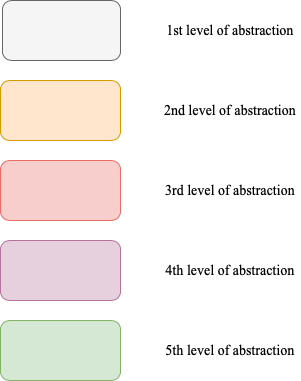
\includegraphics[width=0.5\linewidth]{Figures/Conceptual Model/Legend.png}
	\caption{Legend of levels of abstraction}
	\label{fig:Legend}
\end{figure}

At the summit of the structure stands the entity \emph{Actor}. It embodies a fundamental concept in the field of human-computer interaction, where it is usually considered as a human. In literature it has been defined "as a placeholder for an object when specifying behavior" \cite{de_troyer_conceptual_2007}, i.e. it becomes a way to qualify an abstract object as a system capable of performing actions, stimulating, interacting or reacting to user behavior. The structural model of the XRM Conceptual Model distinguishes in the second abstraction level two macro-categories of Actors as shown in \autoref{fig:ActorHumanNonHuman}.

\begin{figure}[h]
	\centering
	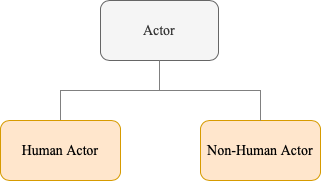
\includegraphics[width=7.5cm]{Figures/Conceptual Model/Actor_Human_NonHuman.png}
	\caption{Structural Model: first two levels of the hierarchy}
	\label{fig:ActorHumanNonHuman}
\end{figure}

\subsection*{Human Actor}
The Human Actor is a type of actor that is generally considered only as a component of the system whose characteristics are crucial in the design process of the interaction with the machine \cite{bannon_discovering_1989}. The presence of a distinction of the Actor between Human and Non-Human arises from the need to elevate the Human from a passive element to an element able to act in an environment, embody and manage a behaviour, rather than being a mere producer of an output information flow. In an interactive system, the Human Actor is nonetheless than the user, the one who uses an application, a device or any technological system through which they perform actions. 

\subsection*{Non-Human Actor}
The Non-Human Actor collects different types of actors, each one with characteristics that must be specified at the design stage. With this term we want to include all the technological components of a system that participate in the interaction allowing the Human Actor to perform certain actions. The results of the interaction are also visible on them.  We can recognize three main sub-categories of Non-Human Actors (\autoref{fig:NonHumanActors}) together with their properties: Physical Component, Environment and Virtual Object.

\begin{figure}[H]
	\centering
	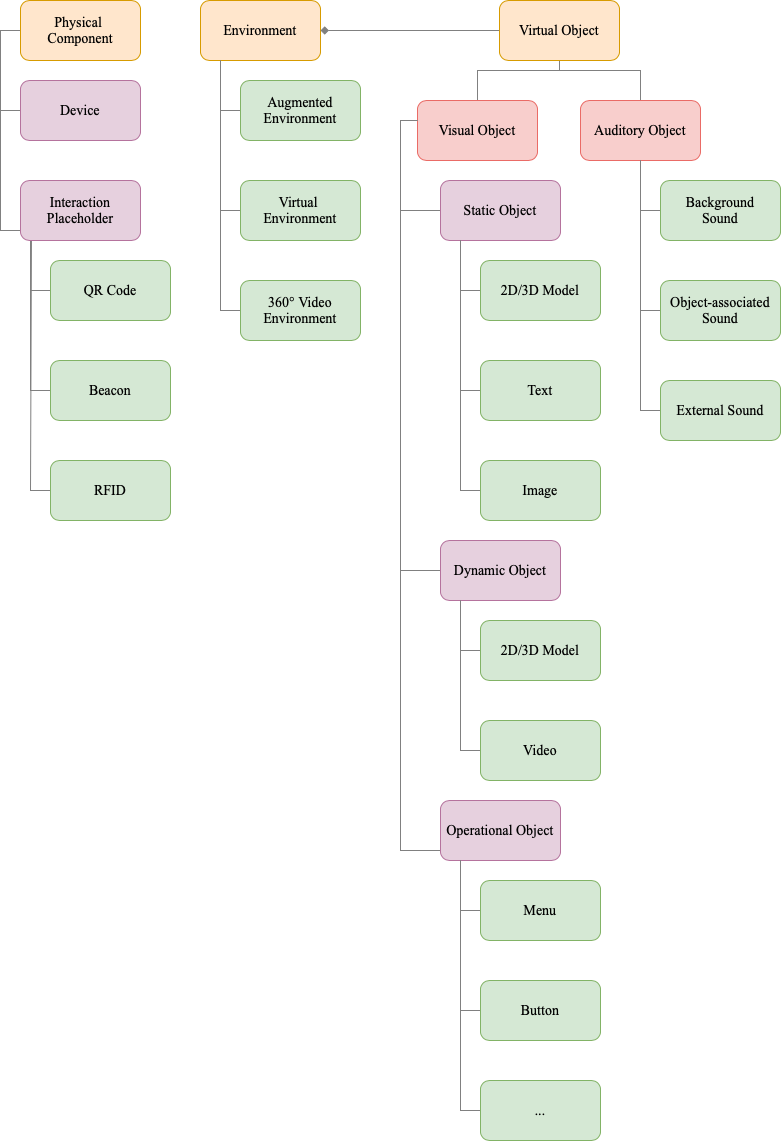
\includegraphics[width=14cm]{Figures/Conceptual Model/NonHumanActors.png}
	\caption{Structural Model - Non-Human Actors hierarchy}
	\label{fig:NonHumanActors}
\end{figure}

\begin{itemize}
    \item \textbf{Physical Component}. Physical Components represent interactive elements with an entirely physical nature, therefore belonging to the real world. They can generate system events or participate in user interactions, receive user commands, trigger other events, etc. \\
    \begin{table}[H]
    \centering
    \begin{tabular}{|l|l|}
    \hline
    \multicolumn{2}{|l|}{\textbf{Physical Component Properties}}                                                                                                \\ \hline
    Id       & It is a unique identification code.                                                                                                              \\ \hline
    Position & \begin{tabular}[c]{@{}l@{}}It is identified by spatial coordinates $(x, y, z)$\\ that locate and track the position of the component.\end{tabular} \\ \hline
    \end{tabular}
    \caption{Structural Model - Physical Component Properties}
    \label{tab:PHCproperties}
    \end{table}
        
    There are two types of Physical Components that we have found:
    \begin{itemize}
        \item \textbf{Interaction Placeholder}. Interaction Placeholders include all identifiable elements i.e. images, codes, symbols such as the QR Code that are recognized by the camera of the device in order to trigger an effect on another Non-Human Actor. However, other devices such as Beacons and RFIDs are also included in this category.
        \item \textbf{Device}: Devices are represented by all the Physical Components that can run an application in XR, whether it is VR or AR. They can be of different nature depending on the technology involved in the designed experience. One or more devices can be included depending on the interaction to be performed. Examples include smartphones, tablets, viewers, card-boards, HMDs, etc.
    \end{itemize}
    \item \textbf{Environment}: Environment represents an element that can have a dual nature. It can identify the real world that can be made of physical objects combined with virtual ones. Otherwise, it can be represented by a world seen through a networked application, a tool supported by a device chosen according to the type of experience designed for the user. In the latter case, the Environment is characterized by a fundamental element: the camera, a device that captures and shows the world to the player. Often the Environment, independently from its nature, is identified with the term "scene", in other cases, instead, the word scene is used to identify the different sub-parts in which it is divided. In this model we will always use only the term 'Environment' in order to avoid any ambiguity. \\
    \begin{table}[H]
    \centering
    \begin{tabular}{|l|l|}
    \hline
    \multicolumn{2}{|l|}{\textbf{Environment Properties}} \\ \hline
    \begin{tabular}[c]{@{}l@{}}Camera \\ Position\end{tabular} &
      \begin{tabular}[c]{@{}l@{}}It is identified by spatial coordinates ($x, y, z$) \\ that locate and track the position of the camera.\end{tabular} \\ \hline
    \begin{tabular}[c]{@{}l@{}}Camera \\ Orientation\end{tabular} &
      \begin{tabular}[c]{@{}l@{}}It is identified by polar coordinates ($\rho$, $\phi$, $\gamma$) \\ that locate and track the camera orientation.\end{tabular} \\ \hline
    Visibility &
      \begin{tabular}[c]{@{}l@{}}It enables or disables the possibility for the user \\ to see the Environment. When in Off mode, the \\ Environment has been triggered but is not visible, \\ i.e. it is hidden from the user's view.\end{tabular} \\ \hline
    \end{tabular}
    \caption{Structural Model - Environment properties}
    \label{tab:Envproperties}
    \end{table}

    The Environment element has three sub-categories:
    \begin{itemize}
        \item \textbf{Augmented Environment}. Augmented Environment (AE) places virtual components in a physical environment. Anchors are virtual elements that the software associates with real elements and that it can recognise, and thus build the experience around the real world by integrating it with the virtual one. Furthermore, AE encapsulates the concept of physical (external) space dimensions, represented as coordinates. It also adds three dimensions where otherwise there would only be one layer superimposed on the users' camera.\\
        \begin{table}[H]
        \centering
        \begin{tabular}{|l|l|}
        \hline
        \multicolumn{2}{|l|}{\textbf{Augmented Environment Properties}}                                                     \\ \hline
        World Anchors & \begin{tabular}[c]{@{}l@{}}They are used by the AR experience\\ to locate the content.\end{tabular} \\ \hline
        \end{tabular}
        \caption{Augmented Environment Properties}
        \label{tab:AEproperties}
        \end{table}
        
        \item \textbf{Virtual Environment}. Virtual Environment  is a completely digital environment that has the characteristic to be navigated and interacted with by the users, of which one or more of their five senses are simulated in real-time \cite{guttentag_virtual_2020}. It places the virtual objects  according to a pure virtual concept of dimensions.
        \begin{table}[H]
        \centering
        \begin{tabular}{|l|l|}
        \hline
        \multicolumn{2}{|l|}{\textbf{Virtual Environment Properties}}                                                       \\ \hline
        World Anchors & \begin{tabular}[c]{@{}l@{}}They are used by the VR experience\\ to locate the content.\end{tabular} \\ \hline
        \end{tabular}
        \caption{Virtual Environment Properties}
        \label{tab:VEproperties}
        \end{table}
        \item \textbf{360$^{\circ}$ Video Environment}. 360$^{\circ}$ Video Environment is represented by a VE that can only be navigated by rotating the device and interacted by buttons superimposed onto the video. The position of the user cannot be changed and overlaps with the position of the camera.\\
        \begin{table}[h]
        \centering
        \begin{tabular}{|l|l|}
        \hline
        \multicolumn{2}{|l|}{\textbf{360$^{\circ}$ Video Environment Properties}}                                           \\ \hline
        Duration & \begin{tabular}[c]{@{}l@{}}It indicates the amount of time\\ the 360$^{\circ}$ Video takes.\end{tabular} \\ \hline
        \end{tabular}
        \caption{360$^{\circ}$ Video Environment Properties}
        \label{tab:360VEproperties}
        \end{table}
    \end{itemize}
    \item \textbf{Virtual Object}. Virtual Object compose the Environment and represent computer-generated elements that simulate real elements and with which the user can interact. Virtual Object in the hierarchy shown (\autoref{fig:NonHumanActors}) is linked to Environment by a "part of" relationship which, as mentioned above, is meant to emphasize that an entity is composed of sub-entities.\\
    \begin{table}[ht]
    \centering
    \begin{tabular}{|l|l|}
    \hline
    \multicolumn{2}{|l|}{\textbf{Virtual Object Properties}}  \\ \hline
    \multirow{4}{*}{Position} &
      \begin{tabular}[c]{@{}l@{}}It is identified by spatial coordinates that \\ locate and track the position of the Virtual Object. \\ These coordinates can be of three types:\end{tabular} \\ \cline{2-2} 
     & Absolute ($x$, $y$, $z$)                               \\ \cline{2-2} 
     & Component-related ($\Delta x$, $\Delta y$, $\Delta z$) \\ \cline{2-2} 
     & User-related ($\Delta x$, $\Delta y$, $\Delta z$)      \\ \hline
    Orientation &
      \begin{tabular}[c]{@{}l@{}}It is identified by polar coordinates ($\rho$, $\phi$, $\gamma$) that \\ locate and track the orientation of the Virtual Object.\end{tabular} \\ \hline
    \end{tabular}
    \caption{Virtual Object Properties}
    \label{tab:VOproperties}
    \end{table}
    Virtual Objects have an additional level of abstraction that characterizes them qualitatively, that is, according to their visual or auditory qualities:
   
   \textbf{Visual Object}. Visual Object encloses a set of Virtual Objects that react to interaction with the user by mainly changing their external characteristics.
    \begin{longtable}[c]{|l|l|l|}
    \hline
    \multicolumn{3}{|l|}{\textbf{Visual Object Properties}} \\ \hline
    \endhead
    %
    \multicolumn{2}{|l|}{Geometry} &
      \begin{tabular}[c]{@{}l@{}}It refers to the representation of the surface, \\ based on mathematical coordinates, that an object \\ can assume. Depending on whether it takes on two or three \\ dimensions, it is called 2D or 3D geometry respectively.\end{tabular} \\ \hline
    \multicolumn{2}{|l|}{Visibility} &
      \begin{tabular}[c]{@{}l@{}}It enables or disables the possibility for the user to see a \\ Visual Object. When in Off mode, the Visual Object has \\ been triggered but is not visible, i.e. it is hidden from \\ the user's view.\end{tabular} \\ \hline
    \multicolumn{2}{|l|}{Scale Factor} &
      \begin{tabular}[c]{@{}l@{}}spatial coordinates (x, y, z) that allow to reduce or increase \\ the size of a Visual Object.\end{tabular} \\ \hline
    \multicolumn{2}{|l|}{Opacity} &
      \begin{tabular}[c]{@{}l@{}}It increases or decreases in percentage the possibility for \\ the user to see a Visual Object. When set to 100\%, the \\ Visual Object has been triggered but is not visible, \\ i.e. it is hidden from the user's view.\end{tabular} \\ \hline
    \multicolumn{2}{|l|}{Selectable} &
      \begin{tabular}[c]{@{}l@{}}It enables or disables the possibility for the user to interact \\ with a Visual Object if the design requires that the object be \\ selected before an action can be performed. When in Off mode, \\ the Visual Object is visible but not interactive, \\ i.e. it does not respond to user commands.\end{tabular} \\ \hline
    \multicolumn{2}{|l|}{Blinking} &
      \begin{tabular}[c]{@{}l@{}}It enables or disables the possibility for the user to see a \\ Visual Object surrounded by a luminous border. When in \\ Off mode, the Visual Object is visible but the luminous border \\ is hidden from the user. This is used, for example, to draw the \\ user's attention to a certain object.\end{tabular} \\ \hline
     &
      Frequency &
      \begin{tabular}[c]{@{}l@{}}It determines the number of times the Visual Object blinks \\ per unit of time.\end{tabular} \\ \hline
     &
      Colour &
      \begin{tabular}[c]{@{}l@{}}It represents the chromatic shade that the light around the \\ Visual Object takes on.\end{tabular} \\ \hline
    \caption{Visual Object Properties}
    \label{tab:VIOtable}\\
    \end{longtable}
    Visual Objects are divided into three subsets: 
    \begin{itemize}
        \item \textbf{Static Object}. Static Object is a Visual Object that is not characterised by movement or animation. We distinguish three types of Static Objects:
        \begin{itemize}
            \item \textbf{2D/3D Model}: 2D/3D Model is a mathematical representation of a two- or three-dimensional object, i.e. a 2D/3D computer-generated geometry.
            \begin{table}[h]
            \centering
            \begin{tabular}{|l|l|}
            \hline
            \multicolumn{2}{|l|}{\textbf{2D/3D Model Properties}} \\ \hline
            Texture &
              \begin{tabular}[c]{@{}l@{}}It is a two-dimensional image in raster format that is \\ reproduced on one or more faces of a multidimensional model. \\ It corresponds to the chromatic variations \\ that a Model may present on the surface.\end{tabular} \\ \hline
            \end{tabular}
            \caption{2D/3D Model Properties}
            \label{tab:2d3dMproperties}
            \end{table}
            \item \textbf{Image}: Image is a visual representation enclosed in a two-dimensional window
            \item \textbf{Text}: Text is a visual description enclosed in a two-dimensional window.\\
            \begin{table}[H]
            \centering
            \begin{tabular}{|l|l|}
            \hline
            \multicolumn{2}{|l|}{\textbf{Text Properties}} \\ \hline
            Offset &
              \begin{tabular}[c]{@{}l@{}}it increases or decreases the user's ability \\ to see Text. When Offset is not set to 100\%, \\ the Text has been triggered but is not visible in full, \\ i.e. a portion is hidden from the user's view.\end{tabular} \\ \hline
            Language &
              \begin{tabular}[c]{@{}l@{}}It allows the user to switch the translation of the \\ Text based on user preferences.\end{tabular} \\ \hline
            \end{tabular}
            \caption{Text Properties}
            \label{tab:Textproperties}
            \end{table}
        \end{itemize}
        \item \textbf{Dynamic Object}. Dynamic Object is a Visual Object that is characterised by movement or animation.\\
        \begin{table}[H]
        \centering
        \begin{tabular}{|l|l|}
        \hline
        \multicolumn{2}{|l|}{\textbf{Dynamic Properties}}                                                                        \\ \hline
        Loop     & \begin{tabular}[c]{@{}l@{}}It enables the cyclic reproduction of a \\ Dynamic Object.\end{tabular} \\ \hline
        Duration & \begin{tabular}[c]{@{}l@{}}It keeps updates the amount of play time of a \\ Dynamic Object.\end{tabular}        \\ \hline
        \end{tabular}
        \caption{Dynamic Properties}
        \label{tab:Dynproperties}
        \end{table}
        There are two types of Dynamic Objects:
        \begin{itemize}
            \item \textbf{2D/3D Model}. 2D/3D Model is a mathematical representation of a two-dimensional/three-dimensional object, i.e. a 2D/3D computer-generated geometry.
            \item \textbf{Video}. Video is a visual reproduction represented in a two-dimensional window.
        \end{itemize}
        \item \textbf{Operational Object}. Operational Object is a Visual Object that allows operations to be carried out and commands to be sent to the system by the user. There are two examples of Operational Objects:
        \begin{itemize}
            \item \textbf{Menu}. Menu consists of a list of elements that can trigger a change of state through a graphical interface, whose geometry can be either 2D or 3D.
            \item \textbf{Button}: Button is a component of the Menu, it allows the user to trigger an event.
        \end{itemize}
    \end{itemize}
    
    \textbf{Auditory Object}. Auditory Object encloses a set of objects that react to interaction with the user with a change in their sound characteristics.\\
	\begin{table}[H]
    \centering
    \begin{tabular}{|l|l|}
    \hline
    \multicolumn{2}{|l|}{\textbf{Auditive Properties}}                                                                                      \\ \hline
    Mute &
      \begin{tabular}[c]{@{}l@{}}It enables or disables the possibility for the user \\ to listen to an Auditory Object. When in Off mode, \\ the Auditory Object has been triggered but cannot \\ be listened to.\end{tabular} \\ \hline
    Duration & \begin{tabular}[c]{@{}l@{}}It allows the user to switch the language of the \\ sound based on user preferences.\end{tabular} \\ \hline
    Loop     & It enables the cyclic playback of an Auditory Object.                                                                        \\ \hline
    \end{tabular}
    \caption{Auditive Properties}
    \label{tab:Audproperties}
    \end{table}
    Auditory Objects are distinguished on the basis of the source from which the sound is reproduced:
    \begin{itemize}
        \item \textbf{Background Sound}: Background Sound is a secondary sound that is activated to complement the experience or part of it, it can be for example a soundtrack etc.
        \item \textbf{Object-associated Sound}: Object-associated Sound is a sound that is linked to the object with which the user is interacting, it can be for example a short sound that provides feedback to indicate the status of the action carried out, such as a timer that signals that time is up.
        \item \textbf{External Sound}: External Sound is a sound from a third party source such as the voice of the tour guide etc.
    \end{itemize}
\end{itemize}

\section{Behavioral Model}
\label{sec:conceptual-behavioral}
\chapter{The ART Framework}
\label{ch:art}

\section{System Overview}
\label{sec:art-overview}

The system architecture of the ART XRaaS is composed by different modules, each reflecting a phase of the creation process of an \gls{XR} experience (\autoref{fig:architecture}). The system is composed as follows:
\begin{itemize}
    \item A \textbf{Content Management System} (CMS) implements the \emph{assets upload phase}. It is a web application acting as entry point into the creation process, where designers of the \gls{XR} experience create or open an existing project and upload all the digital contents to be included in the next phases. It is served by a database to persist and retrieve assets, which can be 3D models (\textit{.fbx, .obj}), images or textures (\textit{.jpeg, .bmp, .png}), video clips (\textit{.mp4}), audio tracks (\textit{.mp3}), text documents (\textit{.txt}), QR Codes (described by their plain text content) and object-related operational entities (a \textit{menu}). Lastly, the application allows to categorize and label these assets, assigning them to different \emph{Scenes}.

    \item The \textbf{ART Editor} is involved in the \emph{interaction authoring phase}. It is a web application that, after retrieving all the assets already uploaded in the previous phase, allows to model in a canvas the interactions among these entities according to user inputs, using a "state-action-effect" paradigm typical of Finite State Machines (FSM). Indeed, the experience is described by a sequence of States connected by Actions, where each State contains different objects and each object has specific properties that can change. After modeling the interactions, the Editor allows to save the flow of the experience in a configuration file used in the next phase.
    
    \item A \textbf{\gls{HMD} Authoring Application} allows the \emph{on-site authoring phase}: during this phase the user, wearing a \gls{HMD}, opens the created project and a \emph{run-time engine} parses the configuration file exported in the previous phase; then, the application downloads all the assets from the CMS' database to proceed in the authoring process. During this phase the authors of the experience set each Scene, placing the assets in the virtual environment and configuring their properties such as position, scale and orientation; in the case of \gls{AR} authoring they map the coordinates of the physical environment with the digital one through \emph{Spacial Anchors}\footnote{\url{https://azure.microsoft.com/en-us/services/spatial-anchors/}} to persist the coordinates of digital contents with respect to real environment. 
    
    \item The on-site authoring phase is the last phase of the development process and, for complimentary, here we cite the last component of the system, that is the \textbf{Universal \gls{XR} Application Reader}. This is the final application for the end user (the tourist) that consists in a run-time engine responsible for the correct parse of the configuration file and rendering of the virtual environment. This application is available for both \glspl{HHD} and \glspl{HMD}, and in the latter case both for \gls{AR} and \gls{VR} devices.
\end{itemize}

\begin{figure}[h]
    \centering
    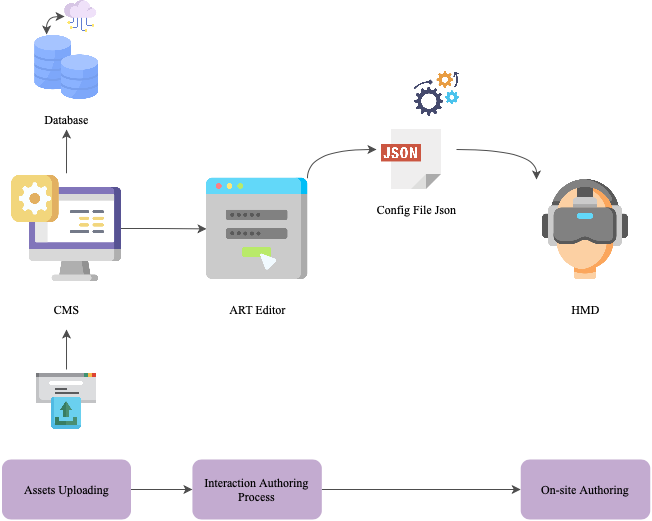
\includegraphics[width=\textwidth]{Figures/Editor/architecture.png}
    \caption{System Overview - Architecture}
    \label{fig:architecture}
\end{figure}

\subsection{ART User Journey}
\label{subsec:art-user-journey}

To give the reader a better understanding of the way the system works we provide a user journey considering the example of a cultural heritage site whose curators are interested in enhancing the experience of their visitors through \gls{XR} technologies. Their goals is to augment the information of the exhibits through virtual panels containing descriptions, historical videos, pictures and reconstruction models of the past; using the ART Framework it is only required some expertise in 3D content authoring to create the models, while the app development part is totally transparent to the user thanks to ART XRaaS. The user journey to develop the \gls{XR} experience would be the following:
\begin{enumerate}
    \item The user produces 3D models and gathers all the digital and multimedia assets contributing to the experience.
    \item The user accesses the web portal of the ART CMS and create a new project.
    \item The user upload all the assets on the CMS, then they define their properties such as names and labels to support the next development phase and, if necessary, cluster each of them in different scenes.
    \item The user opens the ART Editor and define the end user (tourist) interactions with the elements through a canvas and a "state – action – effect" paradigm.
    \item The user save the modelled experience and a configuration file is exported.
    \item The user, wearing a Microsoft HoloLens 2 \gls{HMD}, opens the exported configuration file using the on-site authoring application.
    \item The user decide to create an \gls{AR} application and scan the heritage site to place Spatial Anchors in it; to do so, they place the assets in the environment choosing their placement, size and orientation by manipulating these elements through \emph{gestures}.
    \item Finally, they save and publish the app that will be available for tourists, regardless of the \gls{AR} device used to augment their visit.
\end{enumerate}
\section{ART Editor}
\label{sec:art-editor}

\subsection{From the Conceptual Model to the Editor}
\label{subsec:art-editor-from-conceptual}
\clearpage
\subsection{High-Level Design}
\label{subsec:art-editor-highlevel}

The high-level design of the ART Editor started from an analysis of goals and requirements in projecting and developing an XR application, considering the phases of the framework as described in \autoref{sec:art-overview}. Hence, this study was based on how to specify the run-time behaviour of virtual elements presented in \gls{AR}/\gls{VR} scenes. The goals of the \gls{XR} editor as a component of the ART Framework are:
\begin{itemize}
    \item[\textbf{G1}] The editor supports the design of AR and VR experiences
    \item[\textbf{G2}] The editor allows to model the interactions between users and virtual objects in a scene and the corresponding behaviour of the last ones
    \item[\textbf{G3}] The editor allows to model the interactions and behaviours on elements already uploaded on a Content Management System
    \item[\textbf{G4}] The editor is part of a workflow in the creation of XR experiences and allows to export a modelled environment, as well as load it
    \item[\textbf{G5}] The editor can describe the properties of the elements it supports and their changes
    \item[\textbf{G6}] The editor is based on a syntactically and semantically valid conceptual model
    \item[\textbf{G7}] The editor works on a web application for desktop browsers
\end{itemize}

After having understood which capabilities the XR editor needed to achieve, we started defining the functional requirements to meet during the development of the tool:
\begin{itemize}
    \item[\textbf{R1}] The editor is based on the XRM Conceptual Model
    \item[\textbf{R2}] The editor represents user actions directly on the target elements
    \item[\textbf{R3}] The editor represents elements' run-time properties in 'states' of the application
    \item[\textbf{R4}] The editor allows a flow representation of the interactions
    \item[\textbf{R5}] The editor allows forking and merging of paths in the flow representation for conditional or logic modelling (e.g. logic AND, OR of interactions)
    \item[\textbf{R6}] The editor produces a schema of the modelled experience in order to be read and parsed by the on-site authoring tool
    \item[\textbf{R7}] The editor is able to edit previously modelled experiences
    \item[\textbf{R8}] The editor allows to change the different values of elements only when needed, keeping a clean \gls{UI}
    \item[\textbf{R9}] The editor allows an easy and intuitive UI in order to be used on desktop environments
    \item[\textbf{R10}] The editor allows a technology abstraction modelling
\end{itemize}

\subsubsection*{Editor Specifications}
From the specifications above mentioned and the goals to achieve in order to support the ART Framework in the development of XR applications, we explored the concept (\autoref{fig:art-fsm-sketch}) of an editor representing its elements and their run-time structural properties as a state diagram (\autoref{fig:fsm}) typical of \glspl{FSM}: the behaviour of the application and its virtual objects is described by linked nodes in which user interactions -- corresponding to action nodes -- change the state of these elements, represented in state nodes.
\begin{figure}[h]
    \begin{subfigure}{0.45\columnwidth}
        \centering
        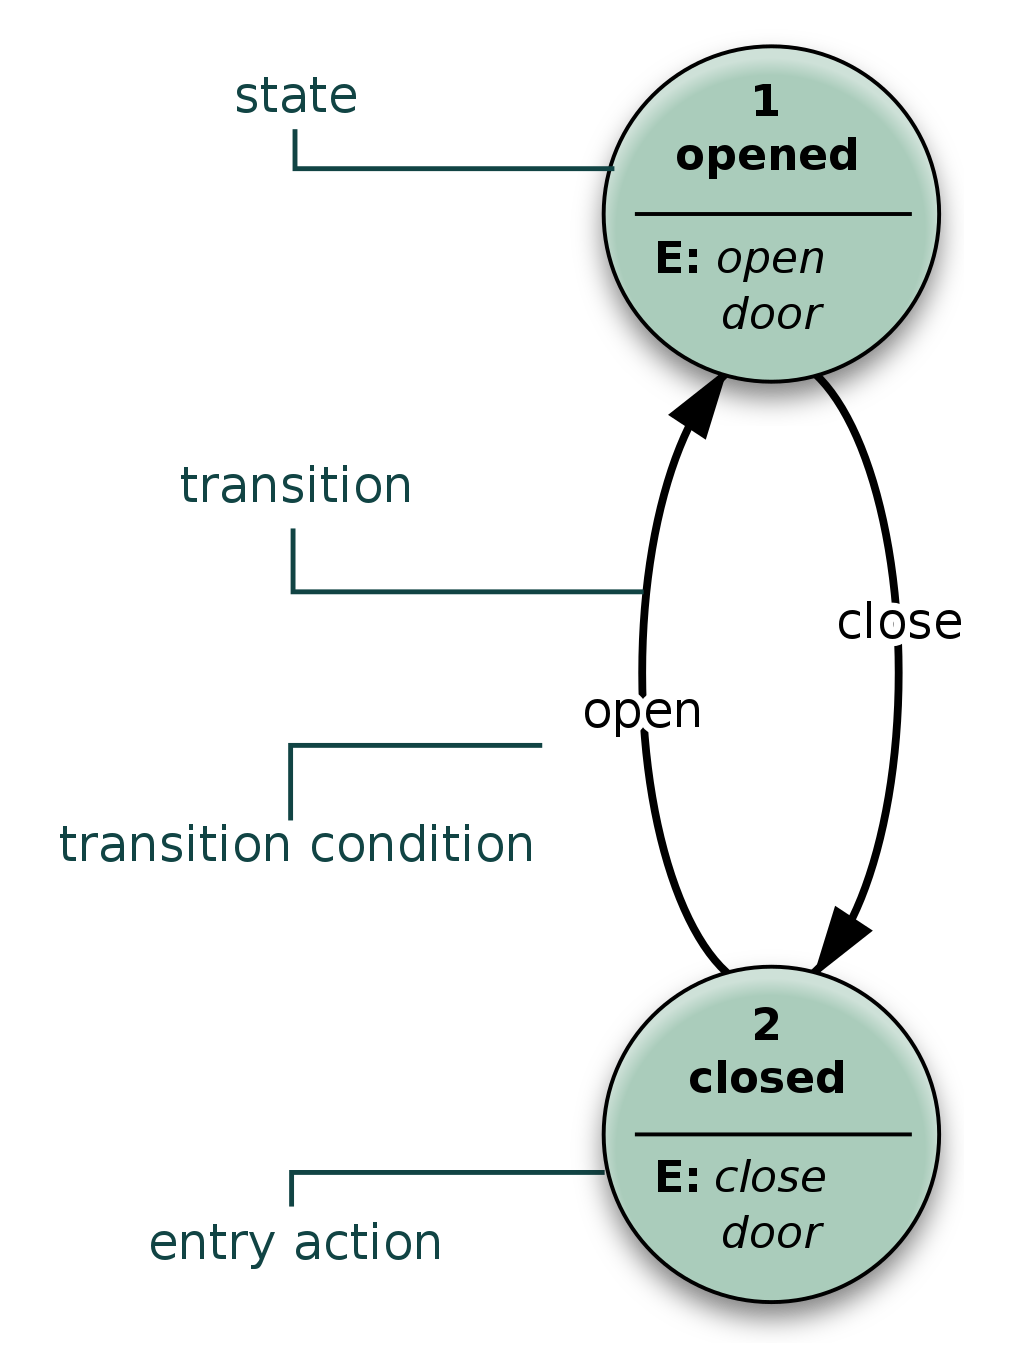
\includegraphics[height=12em]{Figures/Editor/fsm.png}
        \caption{}
        \label{fig:fsm}
    \end{subfigure}
    \begin{subfigure}{0.5\columnwidth}
        \centering
        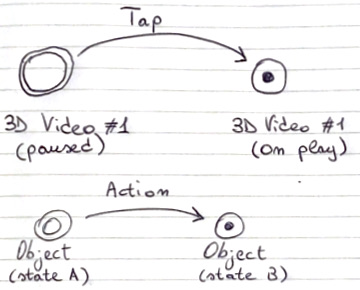
\includegraphics[height=12em]{Figures/Editor/fsm-handwritten.png}
        \caption{}
        \label{fig:art-fsm-sketch}
    \end{subfigure}
    \caption{A door's state diagram (\ref{fig:fsm}) and a handwritten FSM-editor sketch (\ref{fig:art-fsm-sketch})}
\end{figure}

Being a desktop web-application we took full advantage of the web page layout that allows a wider organization of UI components compared to smaller devices (e.g. smartphones); we chose to represent the editor as a blank canvas in which it is possible to draw diagrams representing the XR experience.From the left-hand side panel, all previously loaded assets can be selected as available elements for the editor.
Another feature we thought would allow an easier and cleaner UI is the assignment of actions and properties to elements in the same way -- namely, using a decorator approach to show only relevant property assignments.
Furthermore, the configuration of the modelled experience can be exported, imported and modified using a file describing the diagram, so that it can be supported both by the on-site authoring phase and the interaction authoring phase.

\subsubsection*{Logic Decisions}
The logical high-level design choices consisted of determining the kinds of objects to be modelled in the editor and the actions performed by the user in the interaction. The XRM Conceptual Model in conjunction with the extensive literature review on XR applications in tourism (\autoref{sec:background-tourism-xr}) guided this process, whose first results consisted in choosing the entities (Non-Human Actors) of the XR experience listed in \autoref{table:xrm-art-actors}.

The following step was the definition of the states in which these elements can be distinguished: we decided to cluster the effects on these actors as atomic property modifiers in order to describe as few states as possible for these elements without losing many details in conceptual modelling; for these reasons we found that elements can be in one or more of the following states. \autoref{tab:art-compatible-objects} and \autoref{tab:art-compatible-states} show, respectively, an overview of the available states per entity and the compatibility among different states that can be associated to the same element.

\begin{itemize}
    \item \textbf{Visible} acts on the visibility property -- setting it to 'on' -- and its related opacity
    \item \textbf{Hidden} acts on the visibility property, setting it to 'off'
    \item \textbf{Blinking} enables a luminous border on the target object to attract users' attention
    \item \textbf{Selected} marks the component as selected for more interactions (e.g. manipulation, showing menus, etc.) on it
    \item \textbf{Unselected} deselects the component
    \item \textbf{Manipulated} indicates the component has been manipulated via rotation/translation/scaling
    \item \textbf{On Play} indicates when a multimedia entity is in playback
    \item \textbf{Paused} indicates when a multimedia entity is paused
    \item \textbf{Audio} changes the audio settings, turning it on or off
    \item \textbf{Subtitles} changes the subtitles settings, turning them on or off
\end{itemize}

\begin{table}[h]
\centering
\begin{tabular}{l|c|c|c|c|c|c|c|c|}
\cline{2-9}
 &
  \begin{tabular}[c]{@{}c@{}}3D\\ Scene\end{tabular} &
  \begin{tabular}[c]{@{}c@{}}3D\\ Model\end{tabular} &
  \begin{tabular}[c]{@{}c@{}}3D\\ Video\end{tabular} &
  \begin{tabular}[c]{@{}c@{}}2D\\ Video\end{tabular} &
  \begin{tabular}[c]{@{}c@{}}2D\\ Image\end{tabular} &
  \begin{tabular}[c]{@{}c@{}}2D\\ Text\end{tabular} &
  \begin{tabular}[c]{@{}c@{}}360°\\ Video\end{tabular} &
  Menu \\ \hline
\multicolumn{1}{|l|}{Visible}     & x & x & x & x & x & x & x & x \\ \hline
\multicolumn{1}{|l|}{Hidden}      & x & x & x & x & x & x & x & x \\ \hline
\multicolumn{1}{|l|}{Blinking}    &   & x & x & x & x & x &   & x \\ \hline
\multicolumn{1}{|l|}{Selected}    &   & x & x & x & x & x &   & x \\ \hline
\multicolumn{1}{|l|}{Unselected}  &   & x & x & x & x & x &   & x \\ \hline
\multicolumn{1}{|l|}{Manipulated} &   & x &   &   &   &   &   &   \\ \hline
\multicolumn{1}{|l|}{On Play}     &   &   & x & x &   &   &   &   \\ \hline
\multicolumn{1}{|l|}{Paused}      &   &   & x & x &   &   &   &   \\ \hline
\multicolumn{1}{|l|}{Audio}       &   &   & x & x &   &   & x &   \\ \hline
\multicolumn{1}{|l|}{Subtitles}   &   &   & x & x &   &   & x &   \\ \hline
\end{tabular}
\caption{Compatible objects with states}
\label{tab:art-compatible-objects}
\end{table}

\begin{table}[h]
    \centering
    \begin{tabular}{l|c|c|c|c|c|}
    \cline{2-6}
     & \multicolumn{1}{l|}{Visible} & \multicolumn{1}{l|}{Hidden} & \multicolumn{1}{l|}{Blinking} & \multicolumn{1}{l|}{Selected} & \multicolumn{1}{l|}{Unselected} \\ \hline
    \multicolumn{1}{|l|}{Visible}     &   & X & \checkmark & \checkmark & \checkmark \\ \hline
    \multicolumn{1}{|l|}{Hidden}      & X &   & X & X & \checkmark \\ \hline
    \multicolumn{1}{|l|}{Blinking}    & \checkmark & X &   & \checkmark & \checkmark \\ \hline
    \multicolumn{1}{|l|}{Selected}    & \checkmark & X & \checkmark &   & X \\ \hline
    \multicolumn{1}{|l|}{Unselected}  & \checkmark & \checkmark & \checkmark & X &   \\ \hline
    \multicolumn{1}{|l|}{Manipulated} & \checkmark & X & \checkmark & \checkmark & X \\ \hline
    \multicolumn{1}{|l|}{On Play}     & \checkmark & X & \checkmark & \checkmark & \checkmark \\ \hline
    \multicolumn{1}{|l|}{Paused}      & \checkmark & \checkmark & \checkmark & \checkmark & \checkmark \\ \hline
    \multicolumn{1}{|l|}{Audio}       & \checkmark & X & \checkmark & \checkmark & \checkmark \\ \hline
    \multicolumn{1}{|l|}{Subtitles}   & \checkmark & X & \checkmark & \checkmark & \checkmark \\ \hline
    \end{tabular}
    \caption{Compatibility among states}
    \label{tab:art-compatible-states}
\end{table}

The interactions, required to model virtual objects' changes of states, have been identified following the same process carried out for object states and inspired by XRM Behavioural Model's User Actions (\autoref{tab:BMUserActions}); starting from the table mentioned above, we chose some User Actions and adapted them to the editor and the entire ART Framework, defining their meaning and the objects on which these actions can be performed (\autoref{tab:art-compatible-actions}):
\begin{itemize}
    \item \textbf{Object Recognition} refers to the recognition of QR Codes by the application
    \item \textbf{Voice Command Recognition} is a specific feature for accessibility purposes (e.g. play a content by voice instead of tapping it)
    \item \textbf{Gesture Recognition} enables the modelling of complex gestures defined during the on-site authoring phase
    \item \textbf{Speech to Text} is the action of dictating a text input to the device
    \item \textbf{Proximity In} is the implicit action by a user approaching a virtual content or 3D Scene area
    \item \textbf{Proximity Out} is the implicit action by a user moving away from a virtual content or 3D Scene area
    \item \textbf{Gaze In} can represent both an implicit or explicit action from a user looking at an entity
    \item \textbf{Gaze Out} is the implicit action from a user averting their gaze from an entity
    \item \textbf{Tap} or Press, Click -- is the explicit action by the user on an entity
    \item \textbf{Pinch} is the usual pinch gesture to, for example, grab an object
    \item \textbf{Swipe} the gesture of moving a hand across a virtual object
    \item \textbf{Look Around} happens when the user moves their gaze, changing the field of view of a 360° Video
    \item \textbf{Hand Waving} is the usual hand waving gesture
\end{itemize}

\begin{longtable}[h]{l|c|c|c|c|c|c|c|c|}
\cline{2-9}
 &
  \begin{tabular}[c]{@{}c@{}}3D\\ Scene\end{tabular} &
  \begin{tabular}[c]{@{}c@{}}3D\\ Model\end{tabular} &
  \begin{tabular}[c]{@{}c@{}}3D\\ Video\end{tabular} &
  \begin{tabular}[c]{@{}c@{}}2D\\ Video\end{tabular} &
  \begin{tabular}[c]{@{}c@{}}2D\\ Image\end{tabular} &
  \begin{tabular}[c]{@{}c@{}}2D\\ Text\end{tabular} &
  Menu &
  Device \\ \hline
\endhead
%
\multicolumn{1}{|l|}{Proximity In}                                                          & x & x & x & x & x & x & x &   \\ \hline
\multicolumn{1}{|l|}{Proximity Out}                                                         & x & x & x & x & x & x & x &   \\ \hline
\multicolumn{1}{|l|}{Gaze In}                                                               & x & x & x & x & x & x & x &   \\ \hline
\multicolumn{1}{|l|}{Gaze Out}                                                              & x & x & x & x & x & x & x &   \\ \hline
\multicolumn{1}{|l|}{Tap}                                                                   &   & x & x & x & x & x & x &   \\ \hline
\multicolumn{1}{|l|}{Pinch}                                                                 &   & x & x & x & x & x & x &   \\ \hline
\multicolumn{1}{|l|}{Swipe}                                                                 &   & x & x & x & x & x &   &   \\ \hline
\multicolumn{1}{|l|}{Hand Waving}                                                           &   & x & x & x & x & x & x &   \\ \hline
\multicolumn{1}{|l|}{\begin{tabular}[c]{@{}l@{}}Voice\\ Command\\ Recognition\end{tabular}} &   &   &   &   &   &   &   & x \\ \hline
\multicolumn{1}{|l|}{\begin{tabular}[c]{@{}l@{}}Gesture\\ Recognition\end{tabular}}         &   &   &   &   &   &   &   & x \\ \hline
\multicolumn{1}{|l|}{\begin{tabular}[c]{@{}l@{}}Speech to\\ Text\end{tabular}}              &   &   &   &   &   &   &   & x \\ \hline
\caption{Compatible objects per action. Look Around (360° Video) and Object Recognition (QR Code) omitted.}
\label{tab:art-compatible-actions}
\end{longtable}

In conclusion, we conceived a high-level schema of the editor by defining entities, states and actions for a state diagram model of the application to be modelled; each action applied to an entity in a given modelled state (i.e. a combination of its properties) carries the application and its elements to another state with different structural properties. The next sections will further describe the technological and design choices and how they have been implemented in a working prototype.
\subsection{Low-Level Design}
\label{subsec:art-editor-lowlevel}
\subsection{Implementation}
\label{subsec:art-editor-implementation}
\subsection{Example of use of ART Editor: The NURE Use Case}
\label{subsec:art-editor-nure-example}
\chapter{Evaluation}
\label{ch:evaluation}

\section{Use case: NURE}
\label{sec:nure}
\section{ART Editor Usability Testing}
\label{sec:usability}

\subsection{Results}
\chapter{Conclusions and Future Works}
\label{ch:conclusions}

In this chapter, you present the conclusions of your thesis and a couple of possible future works to extend your results. First of all, you should briefly repeat the problem you addressed in the thesis. Then, you report your achievements and how they improve the state of the art.

\section{Conclusions}
\begin{example}
In this thesis, we analyzed the problem of ... . We proposed a new approach that ... . We tested this method on ... . Reported results show that our proposal outperforms the state of the art method.
\end{example}

\section{Future works}
\begin{example}
There are several appealing paths for future works. A possible extension could be to ... .
\end{example}


%*****************************************************************
%                            APPENDIX                            
%*****************************************************************

\appendix
\chapter{Appendix}
\label{appendix}

\section{JSON State Diagram Example}
\begin{lstlisting}[caption={JSON State Diagram Example}, label=json-schema-example,basicstyle=\ttfamily\footnotesize]
{
  "ARTRecipeID": "32fcf660-7eb5-4edc-b313-e7731fc37389",
  "Name": "example",
  "Description": "Hello, world!",
  "ListOfObjects": [
    {
      "type": "2d_video",
      "id": 1
    }
  ],
  "ListOfStates": [
    {
      "Name": "state",
      "InitState": true,
      "EndState": false,
      "Objects": [
        {
          "type": "2d_video",
          "id": 1,
          "decorations": [
            {
              "type": "visibility_visible",
              "options": {
                "opacity": "100%",
                "animate": false,
                "duration": 0,
                "wait": 0
              }
            },
            {
              "type": "multimedia_pause",
              "options": {}
            }
          ]
        }
      ],
      "ListOfTransitions": [
        {
          "Name": "action",
          "Inputs": [
            {
              "type": "2d_video",
              "id": 1,
              "decorations": [
                {
                  "type": "event_tap",
                  "options": {}
                }
              ]
            }
          ],
          "NextState": "state2"
        }
      ]
    },
    {
      "Name": "state2",
      "InitState": false,
      "EndState": true,
      "Objects": [
        {
          "type": "2d_video",
          "id": 1,
          "decorations": [
            {
              "type": "multimedia_play",
              "options": {
                "loop": true
              }
            }
          ]
        }
      ],
      "ListOfTransitions": []
    }
  ]
}
\end{lstlisting}


\section{JSON State Diagram NURE Case study}
\begin{lstlisting}[caption={JSON State Diagram NURE Case study}, label=json-schema-NURE,basicstyle=\ttfamily\footnotesize]
{
  "ARTRecipeId": "88f4df4b-8bf2-4fd6-ae1e-f8fa3ec3a8b4",
  "Name": "NURE Case Study",
  "Description": "State Diagram of the NURE Experience case study.",
  "ListOfObjects": [
    {
      "type": "3d_scene",
      "id": 20
    },
    {
      "type": "3d_model",
      "id": 4
    },
    {
      "type": "3d_model",
      "id": 5
    },
    {
      "type": "3d_model",
      "id": 8
    },
    {
      "type": "3d_model",
      "id": 6
    },
    {
      "type": "3d_model",
      "id": 7
    },
    {
      "type": "3d_scene",
      "id": 10
    },
    {
      "type": "menu",
      "id": 2
    },
    {
      "type": "menu",
      "id": 3
    },
    {
      "type": "3d_scene",
      "id": 22
    },
    {
      "type": "3d_model",
      "id": 9
    },
    {
      "type": "3d_video",
      "id": 11
    },
    {
      "type": "qr_code",
      "id": 31
    },
    {
      "type": "menu",
      "id": 32
    },
    {
      "type": "3d_scene",
      "id": 30
    }
  ],
  "ListOfStates": [
    {
      "Name": "state",
      "InitState": false,
      "EndState": false,
      "Objects": [
        {
          "type": "3d_scene",
          "id": 20,
          "decorations": [
            {
              "type": "visibility_visible",
              "options": {
                "opacity": "100%",
                "animate": false,
                "duration": 0,
                "wait": 0
              }
            }
          ]
        },
        {
          "type": "3d_model",
          "id": 4,
          "decorations": [
            {
              "type": "visibility_visible",
              "options": {
                "opacity": "100%",
                "animate": false,
                "duration": 0,
                "wait": 0
              }
            },
            {
              "type": "visibility_blinking",
              "options": {
                "loop": false
              }
            }
          ]
        },
        {
          "type": "3d_model",
          "id": 5,
          "decorations": [
            {
              "type": "visibility_visible",
              "options": {
                "opacity": "100%",
                "animate": false,
                "duration": 0,
                "wait": 0
              }
            },
            {
              "type": "visibility_blinking",
              "options": {
                "loop": false
              }
            }
          ]
        },
        {
          "type": "3d_model",
          "id": 8,
          "decorations": [
            {
              "type": "visibility_visible",
              "options": {
                "opacity": "100%",
                "animate": false,
                "duration": 0,
                "wait": 0
              }
            },
            {
              "type": "visibility_blinking",
              "options": {
                "loop": false
              }
            }
          ]
        },
        {
          "type": "3d_model",
          "id": 6,
          "decorations": [
            {
              "type": "visibility_visible",
              "options": {
                "opacity": "100%",
                "animate": false,
                "duration": 0,
                "wait": 0
              }
            },
            {
              "type": "visibility_blinking",
              "options": {
                "loop": false
              }
            }
          ]
        },
        {
          "type": "3d_model",
          "id": 7,
          "decorations": [
            {
              "type": "visibility_visible",
              "options": {
                "opacity": "100%",
                "animate": false,
                "duration": 0,
                "wait": 0
              }
            },
            {
              "type": "visibility_blinking",
              "options": {
                "loop": false
              }
            }
          ]
        }
      ],
      "ListOfTransitions": [
        {
          "Name": "action",
          "ListOfInputs": [
            {
              "type": "3d_model",
              "id": 6,
              "decorations": [
                {
                  "type": "event_swipe",
                  "options": {}
                }
              ]
            }
          ],
          "NextState": "state2"
        },
        {
          "Name": "action2",
          "ListOfInputs": [
            {
              "type": "3d_model",
              "id": 7,
              "decorations": [
                {
                  "type": "event_swipe",
                  "options": {}
                }
              ]
            }
          ],
          "NextState": "state3"
        },
        {
          "Name": "action3",
          "ListOfInputs": [
            {
              "type": "3d_scene",
              "id": 20,
              "decorations": [
                {
                  "type": "event_proximity_out",
                  "options": {
                    "time": 10
                  }
                }
              ]
            }
          ],
          "NextState": "state6"
        }
      ]
    },
    {
      "Name": "state2",
      "InitState": false,
      "EndState": false,
      "Objects": [
        {
          "type": "3d_model",
          "id": 6,
          "decorations": [
            {
              "type": "visibility_hidden",
              "options": {
                "animate": false,
                "duration": 0,
                "wait": 0
              }
            }
          ]
        }
      ],
      "ListOfTransitions": [
        {
          "Name": "action2",
          "ListOfInputs": [
            {
              "type": "3d_model",
              "id": 7,
              "decorations": [
                {
                  "type": "event_swipe",
                  "options": {}
                }
              ]
            }
          ],
          "NextState": "state3"
        },
        {
          "Name": "action3",
          "ListOfInputs": [
            {
              "type": "3d_scene",
              "id": 20,
              "decorations": [
                {
                  "type": "event_proximity_out",
                  "options": {
                    "time": 10
                  }
                }
              ]
            }
          ],
          "NextState": "state6"
        }
      ]
    },
    {
      "Name": "state4",
      "InitState": true,
      "EndState": false,
      "Objects": [
        {
          "type": "3d_scene",
          "id": 10,
          "decorations": [
            {
              "type": "visibility_hidden",
              "options": {
                "animate": false,
                "duration": 0,
                "wait": 0
              }
            }
          ]
        }
      ],
      "ListOfTransitions": [
        {
          "Name": "action4",
          "ListOfInputs": [
            {
              "type": "menu",
              "id": 2,
              "decorations": [
                {
                  "type": "event_tap",
                  "options": {}
                }
              ]
            }
          ],
          "NextState": "state"
        }
      ]
    },
    {
      "Name": "state5",
      "InitState": true,
      "EndState": false,
      "Objects": [
        {
          "type": "3d_scene",
          "id": 10,
          "decorations": [
            {
              "type": "visibility_visible",
              "options": {
                "opacity": "100%",
                "animate": false,
                "duration": 0,
                "wait": 0
              }
            }
          ]
        }
      ],
      "ListOfTransitions": [
        {
          "Name": "action5",
          "ListOfInputs": [
            {
              "type": "3d_scene",
              "id": 10,
              "decorations": [
                {
                  "type": "event_proximity_out",
                  "options": {
                    "time": 10
                  }
                }
              ]
            },
            {
              "type": "3d_scene",
              "id": 20,
              "decorations": [
                {
                  "type": "event_proximity_in",
                  "options": {
                    "time": 10
                  }
                }
              ]
            }
          ],
          "NextState": "state"
        }
      ]
    },
    {
      "Name": "state3",
      "InitState": false,
      "EndState": false,
      "Objects": [
        {
          "type": "3d_model",
          "id": 7,
          "decorations": [
            {
              "type": "visibility_hidden",
              "options": {
                "animate": false,
                "duration": 0,
                "wait": 0
              }
            }
          ]
        }
      ],
      "ListOfTransitions": [
        {
          "Name": "action",
          "ListOfInputs": [
            {
              "type": "3d_model",
              "id": 6,
              "decorations": [
                {
                  "type": "event_swipe",
                  "options": {}
                }
              ]
            }
          ],
          "NextState": "state2"
        },
        {
          "Name": "action3",
          "ListOfInputs": [
            {
              "type": "3d_scene",
              "id": 20,
              "decorations": [
                {
                  "type": "event_proximity_out",
                  "options": {
                    "time": 10
                  }
                }
              ]
            }
          ],
          "NextState": "state6"
        }
      ]
    },
    {
      "Name": "state6",
      "InitState": false,
      "EndState": false,
      "Objects": [
        {
          "type": "3d_model",
          "id": 4,
          "decorations": [
            {
              "type": "visibility_hidden",
              "options": {
                "animate": false,
                "duration": 0,
                "wait": 0
              }
            }
          ]
        },
        {
          "type": "3d_model",
          "id": 5,
          "decorations": [
            {
              "type": "visibility_hidden",
              "options": {
                "animate": false,
                "duration": 0,
                "wait": 0
              }
            }
          ]
        },
        {
          "type": "3d_model",
          "id": 6,
          "decorations": [
            {
              "type": "visibility_hidden",
              "options": {
                "animate": false,
                "duration": 0,
                "wait": 0
              }
            }
          ]
        },
        {
          "type": "3d_model",
          "id": 7,
          "decorations": [
            {
              "type": "visibility_hidden",
              "options": {
                "animate": false,
                "duration": 0,
                "wait": 0
              }
            }
          ]
        }
      ],
      "ListOfTransitions": [
        {
          "Name": "action8",
          "ListOfInputs": [
            {
              "type": "menu",
              "id": 3,
              "decorations": [
                {
                  "type": "event_tap",
                  "options": {}
                }
              ]
            }
          ],
          "NextState": "state7"
        }
      ]
    },
    {
      "Name": "state7",
      "InitState": false,
      "EndState": false,
      "Objects": [
        {
          "type": "3d_scene",
          "id": 22,
          "decorations": [
            {
              "type": "visibility_visible",
              "options": {
                "opacity": "100%",
                "animate": false,
                "duration": 0,
                "wait": 0
              }
            }
          ]
        },
        {
          "type": "3d_model",
          "id": 9,
          "decorations": [
            {
              "type": "visibility_visible",
              "options": {
                "opacity": "100%",
                "animate": false,
                "duration": 0,
                "wait": 0
              }
            }
          ]
        }
      ],
      "ListOfTransitions": [
        {
          "Name": "action7",
          "ListOfInputs": [
            {
              "type": "3d_model",
              "id": 8,
              "decorations": [
                {
                  "type": "event_tap",
                  "options": {}
                }
              ]
            }
          ],
          "NextState": "state8"
        }
      ]
    },
    {
      "Name": "state8",
      "InitState": false,
      "EndState": false,
      "Objects": [
        {
          "type": "3d_model",
          "id": 9,
          "decorations": [
            {
              "type": "visibility_hidden",
              "options": {
                "animate": false,
                "duration": 0,
                "wait": 0
              }
            }
          ]
        },
        {
          "type": "3d_video",
          "id": 11,
          "decorations": [
            {
              "type": "multimedia_play",
              "options": {
                "loop": true
              }
            },
            {
              "type": "visibility_visible",
              "options": {
                "opacity": "100%",
                "animate": false,
                "duration": 0,
                "wait": 0
              }
            }
          ]
        }
      ],
      "ListOfTransitions": [
        {
          "Name": "action10",
          "ListOfInputs": [
            {
              "type": "qr_code",
              "id": 31,
              "decorations": [
                {
                  "type": "recognition_read",
                  "options": {}
                }
              ]
            }
          ],
          "NextState": "state9"
        },
        {
          "Name": "action12",
          "ListOfInputs": [
            {
              "type": "menu",
              "id": 32,
              "decorations": [
                {
                  "type": "event_tap",
                  "options": {}
                }
              ]
            }
          ],
          "NextState": "state9"
        }
      ]
    },
    {
      "Name": "state9",
      "InitState": false,
      "EndState": true,
      "Objects": [
        {
          "type": "3d_scene",
          "id": 30,
          "decorations": [
            {
              "type": "visibility_visible",
              "options": {
                "opacity": "100%",
                "animate": false,
                "duration": 0,
                "wait": 0
              }
            }
          ]
        },
        {
          "type": "3d_scene",
          "id": 22,
          "decorations": [
            {
              "type": "visibility_hidden",
              "options": {
                "animate": false,
                "duration": 0,
                "wait": 0
              }
            }
          ]
        }
      ],
      "ListOfTransitions": []
    }
  ]
}

\end{lstlisting}

\clearpage
\section{SUS Questionnaire}
\label{appendix:sus}

\newcolumntype{P}{>{\centering\arraybackslash}p{0.75cm}}
\newcolumntype{L}{>{\raggedright\arraybackslash}m{0.2\textwidth}}
\newcolumntype{R}{>{\raggedleft\arraybackslash}m{0.2\textwidth}}

\newcommand{\usetbl}{%
  \begin{tabular}{@{}|*5{P|}@{}}
    \hline
    1 & 2 & 3 & 4 & 5 \\
    \hline
  \end{tabular}
}

\newcommand\prop[1]{%
  \item
  \parbox[t]{0.5\textwidth}{#1}%
  \qquad
  \parbox[t]{0.5\textwidth}{\usetbl}%
}

\hspace*{0.625\textwidth}%
\begin{tabularx}{0.5\textwidth}{@{}LR@{}}
  \textbf{Strongly} & \textbf{Strongly} \\
  \textbf{Disagree} & \textbf{Agree} \\
\end{tabularx}
 
\begin{enumerate}
\prop{I think that I would like to use this system frequently}

\prop{I found the system unnecessarily complex}

\prop{I thought the system was easy to use}

\prop{I think that I would need the support of a technical person to be able to use this system}

\prop{I found the various functions in this system were well integrated}

\prop{I thought there was too much inconsistency in this system}

\prop{I would imagine that most people would learn to use this system very quickly}

\prop{I found the system very cumbersome to use}

\prop{I felt very confident using the system}

\prop{I needed to learn a lot of things before I could get going with this system}


\end{enumerate}


\section{Open Ended Questionnaire}
\label{appendix:openended}
\begin{enumerate}
    \item Please tell us more about what were your main problems during the use of the tool.
    \item Please tell us more about what you liked of the tool.
    \item Any further comment.
    \item Do you have some experience in Augmented Reality/Virtual Reality development?
    \item Do you have a Computer Science background?
\end{enumerate}

\section{Sub-tasks}
\label{appendix:subtasks}
\begin{longtable}{ll}
Task 1 &                              \\ \hline
\endfirsthead
%
\endhead
%
       & 3D Model placement           \\
       & Add Visible tag              \\
       & Action Node with 3D Model    \\
       & Tap Action Tag               \\
       & Link between nodes           \\
       & Linked State Node            \\
       & Add 2D Text                  \\
       & Add Visible tag              \\
       & Keep coherent IDs            \\
       &                              \\
Task 2 &                              \\ \hline
       & 2D Video placement           \\
       & Add Visible tag              \\
       & Action Node with 2D Video    \\
       & Link between nodes           \\
       & Tap Action Tag               \\
       & Final state on play          \\
       & Visible tag options          \\
       & Change label name            \\
       & On play tag options          \\
       & Keep coherent IDs            \\
       &                              \\
Task 3 &                              \\ \hline
       & Add Visible tag              \\
       & Set opacity to 90\%          \\
       & Add 2 Action Nodes           \\
       & Tap Action Tag               \\
       & Final state on play          \\
       & Add Proximity Out tag        \\
       & Link the action backwards    \\
       & Proximity Out tag options    \\
       & On play tag loop option      \\
       & Keep coherent IDs            \\
       &                              \\
Task 4 &                              \\ \hline
       & Change recipe name           \\
       & Add Audio off tag            \\
       & Add Subtitles on tag         \\
       & Add 3D Model                 \\
       & Add 3D Video                 \\
       & Add Proximity Out action tag \\
       & Add Proximity In action tag  \\
       & Add Blink tag                \\
       & Add Hidden tag               \\
       & Keep coherent IDs            \\
       & Save the experience         
\end{longtable}
\chapter*{Acknowledgments}
Here you can insert optionally the acknowledgments for who had a significant importance for the accomplishment of this goal. These acknowledgments are less formal than the ones at the beginning of the thesis and are not listed in the table of contents.

%*****************************************************************
%                         REFERENCE LIST                         
%*****************************************************************

\bibliography{
    Biblio/biblio, 
    Biblio/Background/xr-in-tourism,
    Biblio/Background/conceptual_models,
    Biblio/Background/authoring_tools}

\end{document}